\documentclass[12pt, a4paper]{article}
\usepackage[T1]{fontenc}
\usepackage{geometry, microtype}
\usepackage{amsmath, amssymb, mathtools}
\usepackage{bm, physics, siunitx}
\usepackage[shortlabels]{enumitem}
\usepackage{graphicx, wrapfig}
\usepackage{xcolor}
\usepackage{hyperref}


%\usepackage{jinstpub} %
\usepackage{lineno}
\usepackage{booktabs}

\usepackage{subcaption} % Add this package for subfigures

% BEGIN BIBLIOGRAPHY CONFIGURATION
% --------------------------------------------- %
\usepackage[
    maxcitenames = 2, 
    backend=biber,
    style=numeric,
    sorting=none,
            ]{biblatex}
% had to comment these 3
%\usepackage{../bib/atlasbiblatex}
%\addbibresource{../bib/sources.bib}
%\addbibresource{sources.bib}
\addbibresource{sources.bib}
\renewcommand*{\bibfont}{\small}

%\bibliographystyle{unsrtnat}
% --------------------------------------------- %
% END BIBLIOGRAPHY CONFIGURATION


% BEGIN PACKAGE CONFIGURATION
% --------------------------------------------- %
\graphicspath{{../Images}}
\hypersetup{colorlinks = true, allcolors=blue}
\sisetup{separate-uncertainty=true, exponent-product=\cdot}

\newcommand{\hmargin}{3.5cm}
\newcommand{\vmargin}{3.25cm}
\geometry{top=\vmargin, bottom=\vmargin, left=\hmargin, right=\hmargin}

\renewcommand{\figurename}{Slika}
\renewcommand{\contentsname}{Vsebina}
\renewcommand{\tablename}{Tabela}
%\captionsetup[table]{name=Cuadro}
% --------------------------------------------- %
% END PACKAGE CONFIGURATION


% BEGIN HEADER CONFIGURATION
%--------------------------------------------%
%\setlength{\headheight}{13.6pt}
%\usepackage{fancyhdr, extramarks}
%\pagestyle{fancy}
%
%\fancyhf{}
%\fancyhead[L]{\textit{\firstrightmark}}
%\fancyfoot[C]{\centering \thepage}
%
%\renewcommand{\sectionmark}[1]{
%    \markboth{\thesection. \ #1}
%    {\noexpand\firstsubsectiontitle}
%    \global\firstsubsectionmarktrue}
%\renewcommand{\subsectionmark}[1]{
%    \markright{\thesubsection. \, #1}
%    \iffirstsubsectionmark
%\edef\firstsubsectiontitle{\thesubsection. \, #1}
%\fi
%\global\firstsubsectionmarkfalse}
%\newif\iffirstsubsectionmark
%\def\firstsubsectiontitle{}
%--------------------------------------------%
% END HEADER CONFIGURATION

% BEGIN HEADER CONFIGURATION - better
%--------------------------------------------%
\setlength{\headheight}{13.6pt}
\usepackage{fancyhdr, extramarks}
\pagestyle{fancy}

\fancyhf{}
\fancyhead[L]{\textit{\firstrightmark}}
\fancyfoot[C]{\centering \thepage}

\renewcommand{\sectionmark}[1]{
    \markboth{\thesection. \ #1}
    {\thesection. \ #1} % Set both left and right marks to the section title
}
\renewcommand{\subsectionmark}[1]{
    \markright{\thesubsection. \, #1}
    \iffirstsubsectionmark
\edef\firstsubsectiontitle{\thesubsection. \, #1}
\fi
\global\firstsubsectionmarkfalse}
\newif\iffirstsubsectionmark
\def\firstsubsectiontitle{}
%--------------------------------------------%
% END HEADER CONFIGURATION

% BEGIN CUSTOM MACROS
% --------------------------------------------- %
\definecolor{myMaroon}{RGB}{96,0,6}
\newcommand{\myhref}[2]{\hyperref[#1]{\textcolor{blue}{#2}}}
\newcommand{\myurl}[1]{\textcolor{blue}{\texttt{\url{#1}}}}
\DeclarePairedDelimiter\floor{\lfloor}{\rfloor}  % floor function

\newcommand{\diff}{\mathop{}\!\mathrm{d}}
\renewcommand{\vec}[1]{\bm{#1}}
\newcommand{\mat}[1]{\mathbf{#1}}
\newcommand{\tensor}[1]{\mathsf{#1}}
\newcommand{\uvec}[1]{\hat{\vec{#1}}}
\renewcommand{\grad}{\nabla}

\newcommand{\X}{\mat{X}}
\newcommand{\W}{\mat{W}}
\newcommand{\x}{\vec{x}}
\newcommand{\y}{\vec{y}}
\newcommand{\w}{\vec{w}}
\renewcommand{\b}{\vec{b}}
\newcommand{\z}{\vec{z}}
\renewcommand{\a}{\vec{a}}

\newcommand{\geant}{\textsc{Geant4}\xspace \;}
\newcommand{\caloclouds}{\textsc{CaloClouds}\xspace \;}
\newcommand{\ccedm}{\textsc{CaloClouds~II}\xspace \;}
\newcommand{\cccm}{\textsc{CaloClouds~II~(CM)}\xspace}
\newcommand\norm[1]{\left\lVert#1\right\rVert}

\newcommand{\subgrad}[1]{\grad_{\mspace{-4mu}#1}\mspace{1mu}} % gradient with a subscript
\newcommand{\supgrad}[2]{\grad_{\mspace{-4mu}#1}\mspace{1mu}^{\mspace{-4mu}#2}} % gradient with a subscript and superscript
\newcommand{\chem}[1]{\ensuremath{\mathrm{#1}}}  % for typesetting chemical formulas e.g. PbWO_4
% --------------------------------------------- %
% END CUSTOM MACROS


\begin{document}

% BEGIN TITLE PAGE
% --------------------------------------------- %
\thispagestyle{empty}
\begin{center}

    \definecolor{ul-red}{RGB}{220,29,39}
    \begin{figure}[htb!]
        \centering
        
\includegraphics[width=0.8\linewidth]{Images/logo_fmf2.png}
    \end{figure}
    %\huge{\textsc{Univerza \textit{v Ljubljani}}}\\
    %\LARGE{\textsc{Fakulteta za {\color{ul-red} \textit{Matematiko in Fiziko}}}}\\[1mm]
    \Large{\textsc{Oddelek za fiziko}, FMF, UL, 2023/2024}\\
    \vspace{5mm}
    \huge{\textsc{Seminar}, 3. letnik}\\
    \vspace{5mm}
    \rule{\textwidth}{0.2pt}\\[3mm]
    \LARGE{\textbf{Uporaba Difuzijskih Modelov za Simulacije v Fiziki Visokih Energij}}
    \rule{\textwidth}{0.2pt}

    \vspace{4mm}

    \begin{minipage}[t]{0.90\textwidth}
        \normalsize{\textsc{Avtor:}} \hfill \large{\textsc{Mentor}:}\\
    \large{Dimitrije Pešić} \hfill \large{prof. dr. Borut Paul Ker\v{s}evan}
    \end{minipage}

\end{center}

\vspace{10mm}
\begin{center}
    \textbf{Povzetek}\\[2mm]
    \begin{minipage}[t]{0.85\textwidth}
        V tem seminarju se poglobimo v uporabo difuzijskih modelov v simulacijah visokoenergijske fizike, pri čemer se osredotočamo na njihovo naraščajočo pomembnost in uporabo kot zamenjave za tradicionalne metode Monte Carlo, zlasti na področju trkov delcev in interakcij v velikem hadronskem trkalniku (LHC). S to raziskavo želimo razjasniti teoretične temelje in praktične posledice difuzijskih modelov pri napredku našega razumevanja prvih načel fizikalnih pojavov in premikanju mej znanstvenega raziskovanja. 
        Zaključimo s predstavitvijo konkretne študije, ki vključuje uporabo difuzijskega modela za simulacijo pljuskov delcev na kalorimeterskem detektorju.

    \end{minipage}

    \vspace{10mm}
    \large{Ljubljana, Marec 2024}
\end{center}
% --------------------------------------------- %
% END TITLE PAGE

\newpage
\thispagestyle{empty}
\tableofcontents

%\frontmatter
\newpage
%\mainmatter


%\subsection{Why End-to-End Classification?}
%
%\begin{figure}[htb!]
%        \centering
%        \includegraphics[width=0.8\linewidth]{vector/traditional-pipeline.pdf}
%        \caption{An abstracted traditional particle classification workflow.}
%        \label{fig:traditional-pipeline}
%\end{figure}
%of-mass energy~\cite{lhc}.




% --------------------------------------------- %
% BEGIN UVOD PAGES
\setcounter{page}{1}

\section{Uvod v fiziko visokih energij na LHC}

Simulacije igrajo ključno vlogo na vseh področjih fizike delcev, od začetnih faz načrtovanja detektorjev do kompleksne analize podatkov o trkih. Delujejo kot temeljno orodje za razumevanje in napovedovanje vedenja delcev v kompleksnem okolju eksperimentov na Velikem hadronskem trkalniku (angl.: \textit{Large Hadron Collider} - LHC~\cite{lhc}).

Tradicionalno se je simulacija interakcij delcev zanašala predvsem na metode Monte Carlo (MC), to je računski pristop, ki vključuje naključno vzorčenje za simulacijo različnih pojavov. Te simulacije modelirajo dogodke v trkalniku od začetnega trdega sipanja preko hadronizacije\footnote{Hadronizacija je proces nastanka hadronov iz kvarkov in gluonov.} do podrobnih odzivov sledilnega, kalorimetrskega in mionskega sistema detektorja. Tako podrobno modeliranje je proces, ki zahteva veliko računalniške zmogljivosti. Poleg tega mora biti število simuliranih dogodkov vsaj enako številu zabeleženih trkov, da bi bila naknadna statistična primerjava s podatki o trkih relevantna oziroma dovolj natančna. Kot je opisano v ref.~\cite{GANforfastsim}, so MC simulacije predstavljale pomemben del obremenitve na računalniški mreži LHC (angl.: \textit{Worldwide LHC Computing Grid} - WLCG~\cite{WLCG}), pri čemer napovedi kažejo na znatno povečanje povpraševanja, zlasti ob posodobitvi LHC z visoko svetilnostjo (HL-LHC), načrtovano za leto 2025~\cite{HL-LHC}. \\
Iskanje metod, ki so sposobne izboljšanja natančnosti, hitrosti oz. dosegljive MC statistike za dva velikostna razreda, imajo velik pomen za fizike. Poglobimo se v inovativen pristop — Difuzijski Generativni Modeli — in raziščemo njihov potencial za preoblikovanje tehnik simulacije v kontekstu visokoenergijske fizike (angl.: \textit{high energy physics} - HEP) na LHC. Eden razlogov za raziskovanje uporabe difuzijskih modelov je nedavni porast priljubljenosti teh modelov za industrijske aplikacije (DALL-E, Midjourney, SORA, Imagen, …~\cite{DALL-E, Midjourney, SORRA, Imagen}).


\subsection{Kalorimetrični detektorji}

LHC je sinhrotronski trkalnik, ki trka protone pri izjemno visokih energijah, merjenih v teravoltih. Ob trku nastanejo sekundarni delci, katerih energije in poti zaznavajo specializirani detektorji, kot sta CMS in ATLAS.
Elektromagnetni kalorimetri (ECAL) posebej merijo energijo delcev, ki pri danih energijah v materialu kalorimetra ustvarjajo EM pljuske (preko produkcije elektron-pozitron parov in zavornega sevanja). Pri relevantnih energijah so to samo elektroni in fotoni (za masivnejše delce proces postane pomemben pri mnogo večjih energijah). 

V CMS je osnovna enota ECAL kristal iz svinčevega volframata (angl.: \textit{lead tungstate}) \chem{PbWO_4}, povezan s fotodetektorjem. Ko visokoenergetski delci interagirajo s temi kristali, ustvarijo elektromagnetne pljuske, ki vključujejo nižje energijske fotone, elektrone in pozitrone~\cite{ecal-tdr, Mastnak}.
Ti delci iz pljuskov vzbudijo kristale \chem{PbWO_4}, ki med sprostitvenim procesom oddajajo scintilacijske fotone. Ti fotoni dosežejo pritrjene fotodetektorje, kjer sprožijo sprostitev elektronov preko fotoelektričnega pojava. Električni tok, ki pri tem nastane,\, se dodatno ojača in odraža energijo, ki jo je na začetku deponiral vpadni delec.
%% ŠANTELJ KOMENTAR: "pljuske je lepša beseda"
%% MOJ RESPONSE: CTRL+F spremen vse prhe v pljuske I guess
%%% DONE!

\subsection{Simulacije z Geant4}
\label{sec:Geant4}
S simulacijo želimo za nek tip delca z dano energijo modelirati odziv kalorimetra, na nivoju celic (posameznih kristalov) kalorimetra. V principu generiramo sliko odziva \ref{fig:CalorimeterShower}, kjer vsak kristal predstavlja piksel in odložena energija intenziteto piksla. Simulacije pljuskov kalorimetrov opravljamo s programskim paketom \geant~\cite{Geant4}, ki jo je razvila CERN kolaboracija. Gre za bolj elementaren pristop z uporabo MC metode, kjer definiramo geometrijo našega detektorja in določimo delce (njihovo energijo in začetno smer), nakar simulacija razvija EM pljusek preko tvorbe parov in zavornega sevanja ~\cite{Geantclanek}. 
%
\begin{figure}[htb!]
        \centering
        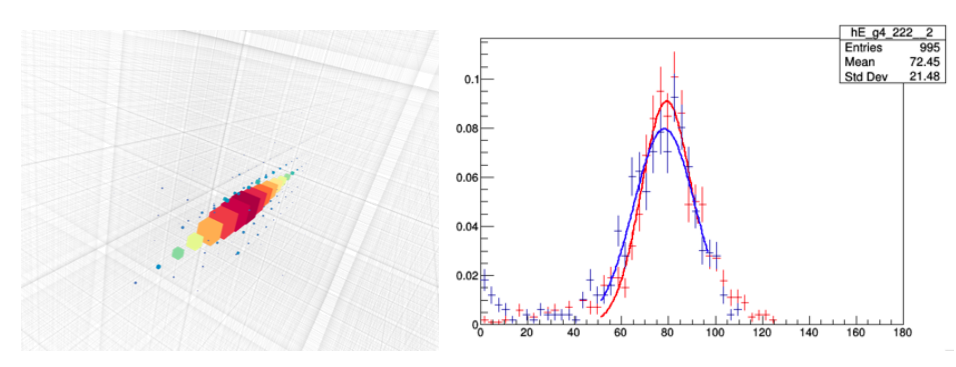
\includegraphics[width=0.95\linewidth]{Images/CalorimeterShower.png}
        \caption{Tipični energijski pljuski, ki jih proizvaja elektron s 100 GeV v ECAL. Sive črte predstavljajo identifikacijo kalorimetrske celice. Barva in dimenzija zadetka ustrezata količini energije, deponirane v celici ~\cite{CalorimeterShower}.}
        \label{fig:CalorimeterShower}
\end{figure}




% --------------------------------------------- %
% END UVOD PAGES

% --------------------------------------------- %
% BEGIN ML PAGES
%\newpage
\section{Osnove strojnega učenja}

\subsection{Nevronske mreže}


Preden se poglobimo v posebnosti difuzijskih modelov, je pomembno da razumemo osnove strojnega učenja, zlasti nevronskih mrež (NN). Nevronsko mrežo sestavljajo trije tipi plasti:
\begin{itemize}
    \item Vhodna plast: začetna plast kamor se dovajajo neobdelani podatki $\bf{x}$.
    
    \item Vmesne plasti: odgovorne za pridobivanje in preoblikovanje funkcij iz vhodnih podatkov z nelinearnimi transformacijami, imenovanimi aktivacijske funkcije. Tipični aktivacijski funkciji sta sigmoidna $\sigma(x) = \frac{1}{1 + e^{-x}}$ in $\text{ReLU}(x) = \max({x, 0})$.
    
    \item Izhodna plast: končna plast, ki vrne napovedi ali rezultate modela na podlagi naučenih povezav iz skritih plasti.
\end{itemize}

\begin{figure}[htb!]
        \centering
        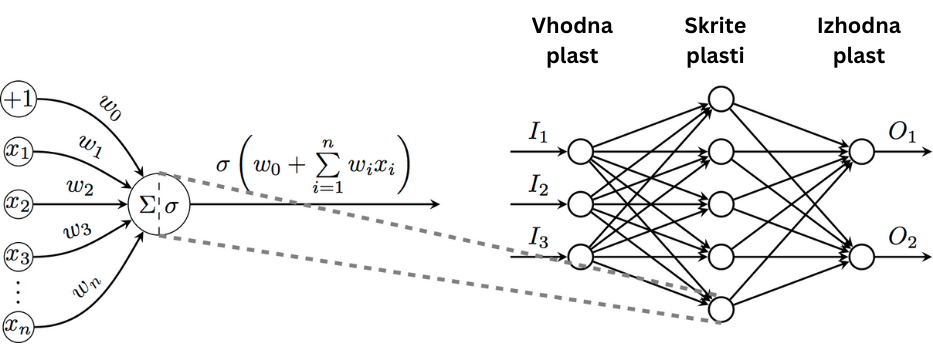
\includegraphics[width=0.8\linewidth]{Images_SLO/Neural Network_SLO.png}
        \caption{Skica posameznega nevrona (levo), skica polno povezane nevronske mreže (desno)~\cite{PetarV}.}
        \label{fig:NN}
\end{figure}

Na sliki \ref{fig:NN} so prikazane posamezne plasti, ter delovanje NN mreže na posameznem nevronu. V vsaki plasti se nevroni prejšnje plasti obteženo seštejejo s povezavami med njimi. Doda se še parameter pristranskosti, označen z $b$ (angl.: \textit{bias}). To le predstavlja afino transformacijo v matematiki, s čimer pa ne moremo modelirati kompleksnejših vzorcev, zato vse skupaj pošljemo skozi prej omenjeno aktivacijsko funkcijo. Postopek ponovimo za vsak sloj, kjer nam sedaj aktivacija prejšnjega sloja predstavlja nov vhod $\bf{x}$.
Za posamezen nevron lahko aktivacijo $a_i$, kjer indeks $i$ predstavlja $globino$ (zaporeden sloj v mreži), indeks $n$ pa posamezen nevron na globini $i$, zapišemo:
\begin{equation}
    a_i = \theta\left(\sum_{n} x_n w_{i,n} + b_i \right)\,,
\end{equation}
kjer $\theta$ predstavlja našo izbiro aktivacijske funkcije.
Vse skupaj lahko opišemo v matrični obliki, uteži zapišemo v obliki matrike $W \in \mathbb{R}^{m\times n}$, $\bf{ b}$ pa vektor pristranskosti:
\begin{equation}
    \bf{a} = \theta\left(W\bf{x} + \bf{b}\right)\,.
\end{equation}

\subsection{Učenje mreže}
\label{sec:NNlearning}

Učenje nevronske mreže vključuje iterativno prilagajanje njenih \textit{parametrov} $\theta_t = (W, b)$ (uteži in pristranskosti), da se minimizira vnaprej določena funkcija izgube $L$ (angl.: \textit{Loss function}), ki kvantificira neskladje med predvidenimi izhodi nevronske mreže in že vnaprej znanim željenim izidom. Fiziki pogosto uporabljamo funkcijo povprečja kvadratov napake (MSE): $L_{MSE} = {1\over N}\sum_{i=1}^N\left(y_i - \hat{y}_i\right)^2$, ki je v neposrednem sorodu, testu $\chi^2$. \\
Ta proces, znan kot povratno širjenje napake (angl.: \textit{backpropagation}), vključuje širjenje gradienta napake nazaj po omrežju in posodabljanje parametrov z uporabo optimizacijskih algoritmov, kot je stohastični gradientni spust (SGD) ali njegove različice:
\begin{equation}
    \theta_{t+1} = \theta_t - \alpha\nabla L(\theta_t)\,,
\end{equation}
kjer $\alpha$ predstavlja korak/hitrost učenja (angl.: \textit{learning rate}).

Pri treniranju je potrebno biti pozoren na pravilno izbiro funkcije izgube za željen cilj, pri SGD nastaja problem lokalnih minimumov, ter past pretreniranja (angl.: \textit{overfitting}) - premale količine testnih podatkov za preveliko število prostih parametrov modela~\cite{SGD, Overfitting}.


\subsection{Konvolucijske mreže}

Konvolucijske nevronske mreže (CNN) so se pojavile kot specializiran razred nevronskih mrež, prilagojenih za obdelovanje slik. Odlične so pri zajemanju prostorskih hierarhij značilk na slikah, zaradi česar so posebej primerne za naloge, kot so klasifikacija slik, zaznavanje objektov in segmentacija. Tipičen prikaz konvolucijske mreže je na sliki \ref{fig:CNN}.
Arhitektura in ključne komponente CNN so:
\begin{itemize}
	\item Konvolucijski sloji: kot ime pove, opravijo konvolucijo slike z jedri (angl.: \textit{kernels}) (znanimi tudi kot filtri), da izluščijo lokalne značilnosti. Konvolucijska operacija vključuje drsenje jedra po vhodni sliki in sumacijo posameznih množenj po elementih (analog uteži v NN). Nastali zemljevidi značilnosti (angl.: \textit{feature maps}) zajemajo vzorce in robove, ki so prisotni na vhodni sliki.
	\item Združevalne plasti (angl.: \textit{pooling layers}): se uporablja za zniževanje dimenzij zemljevidov značilnosti, ob tem pa ohranjanjajo pomembne značilnosti. Združevalne plasti pomagajo pri doseganju translacijske invariantnosti in zmanjševanju računske kompleksnosti (manj parametrov, manjši problem s pretreniranjem)
	\item Polno povezani sloji: Po več konvolucijskih in združevalnih slojih se izluščene funkcije/značilke sploščijo in prenesejo skozi eno ali več popolnoma povezanih plasti - navadna nevronska mreža.
\end{itemize}

\begin{figure}[htb!]
        \centering
        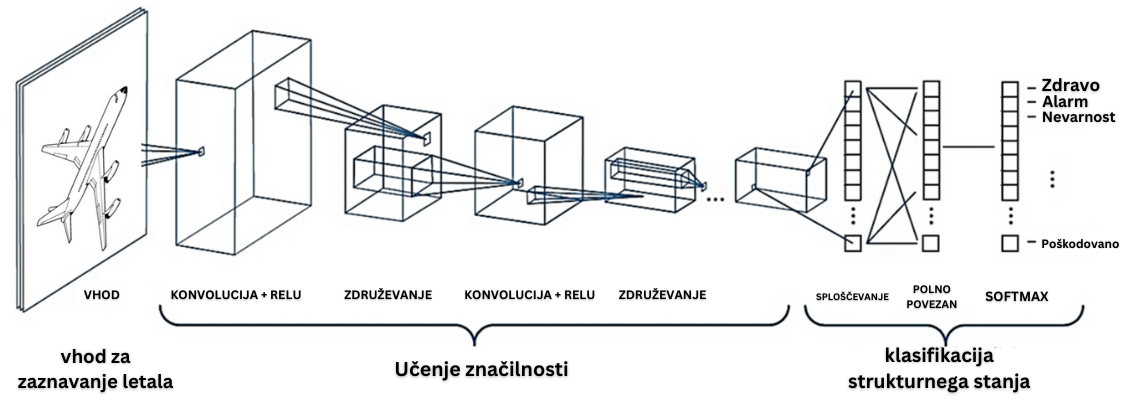
\includegraphics[width=0.7\linewidth]{Images_SLO/CNN2_SLO.png}
        \caption{Skica posameznih nivojev konvolucijske mreže. Slika povzeta z ref.~\cite{CNNim}.}
        \label{fig:CNN}
\end{figure}

% --------------------------------------------- %
% END ML PAGES


% --------------------------------------------- %
% BEGIN GM PAGES
\newpage
\section{Uvod v generativne modele}

Generativni modeli omogočajo ustvarjanje novih vzorcev podatkov, ki tesno spominjajo na originalne podatke. Za razliko od diskriminativnih modelov, ki se osredotočajo na napovedovanje oznak ali klasifikacijo vhodov, se generativni modeli osredotočajo na razumevanje in generiranje podatkov. Nekaj generativnih modelov je prikazanih na sliki \ref{fig:Generative models}.
\begin{figure}[htb!]
        \centering
        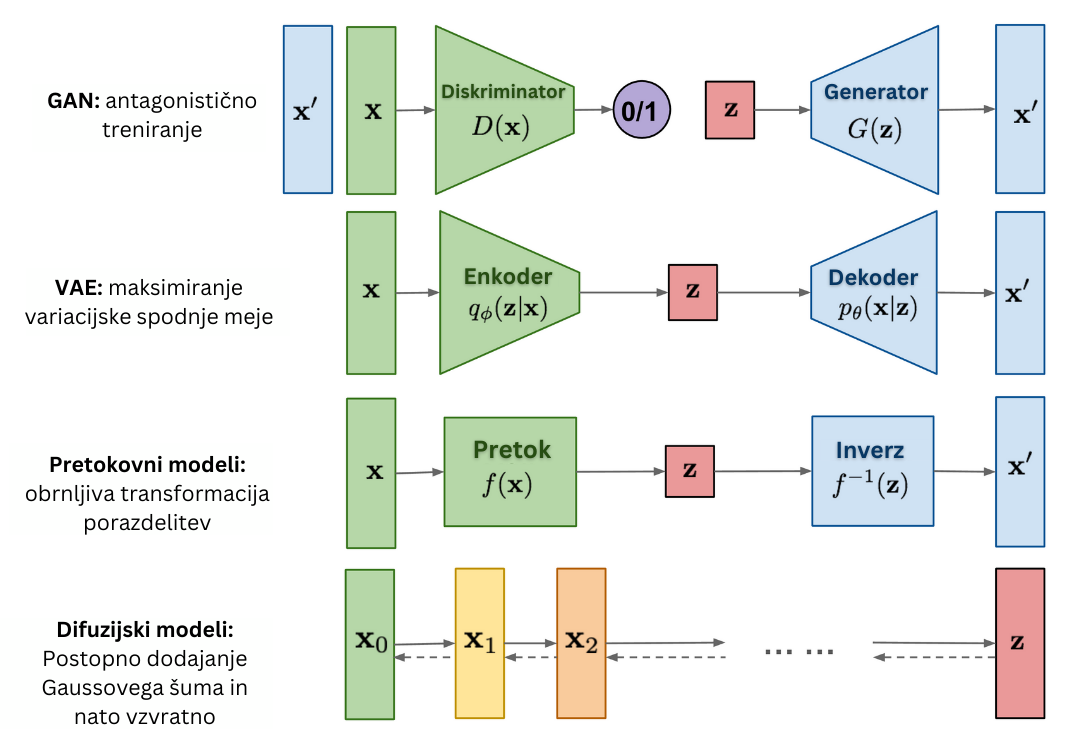
\includegraphics[width=0.8\linewidth]{Images_SLO/generative-overview_SLO.png}
        \caption{Pregled različnih tipov generativnih modelov~\cite{weng2021diffusion}.}
        \label{fig:Generative models}
\end{figure}

Generativne Antagonistične Mreže (angl.: \textit{Generative Adversarial Networks} - GANs) spadajo med ene najbolj priljubljenih modelov. GANs sestavljajo dve nevronski mreži, generator in diskriminator, ki sta vključeni v minimax igro. Generator se uči proizvajati realistične vzorce, medtem ko se diskriminator uči razlikovati med resničnimi in generiranimi vzorci. GANi so pokazali izjemno uspešnost pri generiranju visokokakovostnih slik vendar so nestabilni pri treniranju in so pogosto predmet problema antagonističnih primerov~\cite{antagonist}.

Še en popularen model so Variacijski Avtoenkoderji (VAEs). VAEs modeli se naučijo latentne (prikrite) reprezentacije vhodnih podatkov in generirajo nove vzorce z vzorčenjem iz naučenega latentnega prostora. So hitri pri vzorčenju, enostavni za treniranje, vendar zato na splošno proizvajajo rezultate slabše kvalitete. \\

Poleg modelov, kot so VAEs in GANs, se je pojavil v zadnjih letih nov razred generativnih modelov, ki temeljijo na difuzijskih procesih. Ti modeli, navdihnjeni s teorijo stohastičnih procesov neravnovesne termodinamike~\cite{nonequilibrium-thermodynamics}, izkoriščajo koncept iterativnega izboljševanja porazdelitve šuma za generiranje visokokakovostnih vzorcev.


% --------------------------------------------- %
% END GM PAGES


% --------------------------------------------- %
% BEGIN DM PAGES
%\newpage
\section{Difuzijski modeli}
\label{sec:Diffusion_Models}

Predlaganih je bilo več generativnih modelov, ki temeljijo na difuziji, v tem seminarju se osredotočimo na implementacijo difuzijskih verjetnostnih modelov za zmanjšanje šuma (denoising diffusion probabilistic models - DDPM; Ho et al.~\cite{DDPM}).
V principu so si te implementacije podobne. Najprej definiramo verigo Markova\footnote{Veriga Markova je stohastični model, ki opisuje verjetnost zaporedja dogodkov, ki se zgodi na podlagi prejšnjega dogodka~\cite{Markov-chain}.} difuzijskih korakov za počasno dodajanje naključnega šuma podatkom, modeli pa se nato naučijo obrniti proces difuzije, da iz šuma sestavijo želene vzorce podatkov (slika \ref{fig:forward-reverse-process}).
\begin{figure}[htb!]
        \centering
        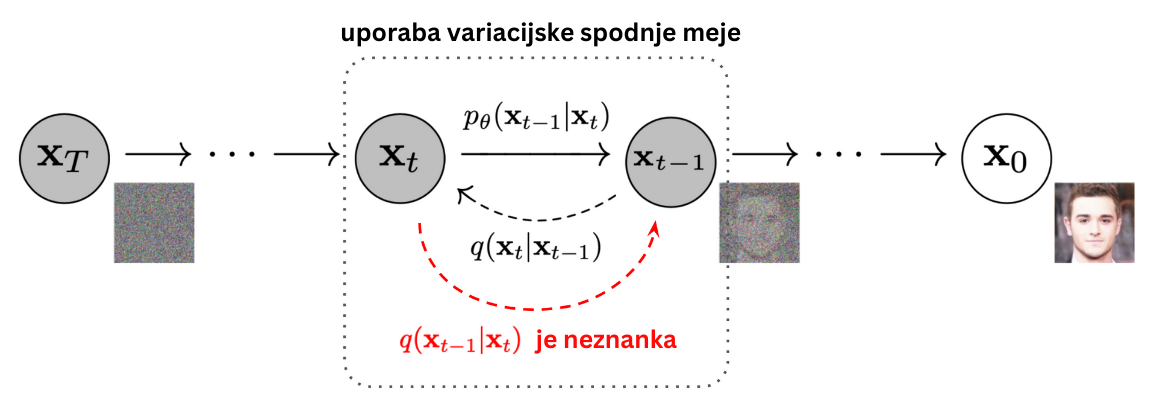
\includegraphics[width=0.7\linewidth]{Images_SLO/DDPM Markov Chain_SLO.png}
        \caption{Markovljeva veriga naprednega (povratnega) difuzijskega procesa generiranja vzorca s počasnim dodajanjem (odstranjevanjem) šuma. (Vir slike: Ho et al.~\cite{DDPM}).}
        \label{fig:forward-reverse-process}
\end{figure}

\subsection{Matematično ozadje}

Na visoki ravni difuzijski modeli vzorčijo iz porazdelitve tako, da obrnejo postopni proces šumljenja. Podroben pregled formulacije Gaussovih difuzijskih modelov iz ref.~\cite{nonequilibrium-thermodynamics, DDPM, DMs-beat-GANs}. Začnemo z definiranjem naše distribucije podatkov $x_0 \sim q(x_0)$ in Markovskega procesa $q$, ki podatkom postopoma dodaja Gaussov šum, da ustvari zašumljene vzorce od $x_1$ do $x_T$. Matematičen zapis tega je:
%
\begin{alignat}{2}
q(x_t|x_{t-1}) &\coloneqq \mathcal{N}(x_t; \sqrt{1-\beta_t}x_{t-1}, \beta_t \mathbf{I}).
\end{alignat}

kjer $x_t$ predtavlja izhod funkcije, $\mathcal{N}$ predstavlja Gaussov šum, ki je vzorčen glede na razpored variance $\beta_t$. Razporejevalnik variance šuma $\beta_t$ nam omogoča apliciranje različne količine šuma glede na časovni/iteracijski korak $t$. V rabi sta najpogostejši linearen in kosinusni, saj omogočita bolj postopno uničenje slike.


Ho et al.~\cite{DDPM} ugotavljajo, da nam ni treba večkrat zaporedoma uporabiti funkcije $q(x_i|x_{i-1})$, za vzorec iz $x_t \sim q(x_t|x_0)$. Namesto tega lahko tudi $q(x_t|x_0)$ izrazimo kot Gaussovo porazdelitev z $\alpha_t \coloneqq 1 - \beta_t$ in $\bar{\alpha}_t \coloneqq \prod_{s=0}^{t} \alpha_s$
%
\begin{alignat}{2}
    q(x_t|x_0) &= \mathcal{N}(x_t; \sqrt{\bar{\alpha}_t} x_0, (1-\bar{\alpha}_t) \mathbf{I}) \\
    x_t(x_0, \epsilon) = x_t &= \sqrt{\bar{\alpha}_t} x_0 + \epsilon \sqrt{1-\bar{\alpha}_t},\quad\text{  } \epsilon \sim \mathcal{N}(0, \mathbf{I}) \label{eq:jumpnoise}
\end{alignat}

Tu nam $1 - \bar{\alpha}_t$ pove varianco šuma za poljuben časovni korak in to bi lahko enakovredno uporabili za definiranje razporeda šuma namesto $\beta_t$.

Z uporabo Bayesovega izreka ugotovimo, da je posteriorni člen $q(x_{t-1}|x_t,x_0)$ prav tako Gaussov s povprečjem $\tilde{\mu}_t(x_t,x_0)$ in varianco $\tilde{ \beta}_t$ definiran kot sledi:
%
\begin{alignat}{2}
    \tilde{\mu}_t(x_t,x_0) &\coloneqq \frac{\sqrt{\bar{\alpha}_{t-1}}\beta_t}{1-\bar{\alpha}_t}x_0 + \frac{\sqrt{\alpha_t}(1-\bar{\alpha}_{t-1})}{1-\bar{\alpha}_t} x_t \label{eq:mutilde} \\
    \tilde{\beta}_t &\coloneqq \frac{1-\bar{\alpha}_{t-1}}{1-\bar{\alpha}_t} \beta_t \label{eq:betatilde} \\
    q(x_{t-1}|x_t,x_0) &= \mathcal{N}(x_{t-1}; \tilde{\mu}(x_t, x_0), \tilde{\beta}_t \mathbf{I}) \label{eq:posterior}
\end{alignat}
Če želimo vzorčiti iz distribucije podatkov $q(x_0)$, lahko najprej vzorčimo iz $q(x_T)$ in nato vzorčimo obratne korake $q(x_{t-1}|x_t)$, dokler ne dosežemo $x_0 $. Pri razumnih nastavitvah za $\beta_t$ in $T$ je porazdelitev $q(x_T)$ skoraj izotropna Gaussova porazdelitev, zato je vzorčenje $x_T$ trivialno. Vse, kar ostane, je aproksimacija $q(x_{t-1}|x_t)$ z uporabo nevronske mreže, saj je ni mogoče natančno izračunati, ko je porazdelitev podatkov neznana. V ta namen~\cite{nonequilibrium-thermodynamics} upošteva, da se $q(x_{t-1}|x_t)$ približa diagonalni Gaussovi porazdelitvi ko $T \to \infty$ in ustrezno $\beta_t \to 0$, torej zadostuje trenirati nevronske mreže (označene z indeksom $\theta$) za napovedovanje povprečja $\mu_{\theta}$ in diagonalne kovariančne matrike $\Sigma_{\theta}$:


%
\begin{alignat}{2}
p_{\theta}(x_{t-1}|x_t) &\coloneqq \mathcal{N}(x_{t-1};\mu_{\theta}(x_t, t), \Sigma_{\theta}(x_t, t))\,. \label{eq:ptheta}
\end{alignat}

Za treniranje tega modela tako, da se $p(x_0)$ nauči prave porazdelitve podatkov $q(x_0)$, lahko optimiziramo kot funkcijo izgube $L$ naslednjo variacijsko spodnjo mejo $L_{\text{vlb}}$ za $p_{\theta} (x_0)$:
%
\begin{alignat}{2}
    L_{\text{vlb}} &\coloneqq L_0 + L_1 + ... + L_{T-1} + L_T\,, \label{eq:loss} \\
    L_{0} &\coloneqq -\log p_{\theta}(x_0 | x_1)\,, \label{eq:loss0} \\
    L_{t-1} &\coloneqq \kld{q(x_{t-1}|x_t,x_0)}{p_{\theta}(x_{t-1}|x_t)}\,, \label{eq:losst} \\
    L_{T} &\coloneqq \kld{q(x_T | x_0)}{p(x_T)}\,. \label{eq:lossT}
\end{alignat}
%


%
Medtem ko je zgornji cilj dobro utemeljen, so v~\cite{DDPM} ugotovili, da drugačen cilj ustvari boljše vzorce v praksi. Zlasti ne parametrizirajo neposredno $\mu_{\theta}(x_t,t)$ kot nevronsko mrežo, ampak namesto tega trenirajo model $\epsilon_{\theta}(x_t,t)$ za napovedovanje $\epsilon$ šuma iz enačbe \ref{eq:jumpnoise}. Ta poenostavljeni cilj ki se lahko izpelje iz razlage difuzijskega modela z odpravljanjem šuma kot VAE je opredeljen s funkcijo izgube:
%
\begin{alignat}{2}
    L_{\text{preprost}} &\coloneqq E_{t \sim [1,T],x_0 \sim q(x_0), \epsilon \sim \mathcal{N}(0, \mathbf{I})}\left[\left||\epsilon - \epsilon_{\theta}(x_t, t)|\right|^2\right]\,, \label{eq:lsimple}
\end{alignat}
% I fucking hate da rabm tole dodat
kjer, kot nam indeksi v formuli nakazujejo, je čas $t\in[1, T]$, $x_0$ iz  začetne distribucije podatkov, $\epsilon\sim\mathcal{N}(0, \bf{I})$ pa šum vzorčen po normalni porazdelitvi. Med vzorčenjem lahko uporabimo substitucijo za izpeljavo $\mu_{\theta}(x_t,t)$ iz $\epsilon_{\theta}(x_t,t)$:
%
\begin{alignat}{2}
    x_{t-1} =\mu_{\theta}(x_t,t) &=  \frac{1}{\sqrt{\alpha_t}}\left(x_t-\frac{1-\alpha_t}{\sqrt{1-\bar{\alpha}_t}}\epsilon_{\theta}(x_t, t)\right) \label{eq:mufromeps}
\end{alignat}

Upoštevajte, da $L_{\text{preprost}}$ ne zagotavlja nobenega signala za učenje variance $\Sigma_{\theta}(x_t,t)$ iz enačbe \ref{eq:ptheta}, tako v ref.~\cite{DDPM} ugotovijo, da namesto učenja $\Sigma_{\theta}(x_t,t)$ lahko to postavijo na konstanto $\beta_t \mathbf{I}$. Vrednost ustreza zgornji in spodnji meji za pravo varianco obratnega koraka.
Treniranje s tem ciljem in uporaba njihovega ustreznega postopka vzorčenja je enakovredno modelu točkovnega ujemanja (angl.: \textit{score matching}) za odpravljanje šumov iz članka Songa in Ermona~\cite{DDIM, improved-DDIM}. Ta model uporablja Langevinovo dinamiko za vzorčenje iz modela za odpravljanje šumov, ki pa presega debato tega seminarja. Pogosto uporabljamo "difuzijski modeli" kot kratico za oba razreda modelov. \\

Skratka, treniramo U-Net arhitekturo \ref{fig:U-Net} (predstavljeno podrobneje v \ref{sec:UNet}) tako, da optimiziramo formulo \ref{eq:lsimple} z uporabo backpropagation algoritma (poglavje \ref{sec:NNlearning}). Ko imamo natreniran model, vzorčimo sliko iz naključnega šuma z uporabo formule \ref{eq:mufromeps}. Shematično je celoten postopek predstavljen na sliki \ref{fig:algorithms} kot psevdokoda algoritmov za treniranje in vzorčenje difuzijskih modelov.

%\newpage
%% ŠANTELJ KOMENTAR: "Tudi tole ne vem, če je posebej relevantno. Osebno, bi raje vel prostora namenil 4.1. kjer bi poskušal osnovno idejo malo bolj jasno predstavit (vsaj, da malo lepše opišete kaj količine, ki v uporabljenih formulah nastopajo so).
%% MOJ RESPONSE: fukn U-net v appendix in referenci, nek quick summary izpeljave
%%% DONE: I think this is good enough.




%\newpage
\subsection{Rezultati}

Z nekaj izboljšavami arhitekture, opisanimi v članku~\cite{DMs-beat-GANs}, avtorji omogočijo difuzijskim modelom, da bistveno prekašajo najboljše GAN modele, hkrati pa ohranijo večjo pokritost distribucije.
Slika \ref{fig:flamingos} primerja naključne vzorce iz najboljšega globokega modela BigGAN z našim difuzijskim modelom v članku~\cite{DMs-beat-GANs}.
Medtem ko so vzorci podobne zaznavne kakovosti, difuzijski model vsebuje več raznolikosti kot model GAN, kot so povečane nojeve glave, posamezni flamingi, različne orientacije hamburgerjev in riba, ki je ne drži človek. Metrika, ki se uporablja za oceno kakovosti slik, ustvarjenih z generativnim modelom se imenuje FID - Fréchetova začetna razdalja (angl.: \textit{Fréchet inception distance})~\cite{FID}.

\begin{figure}[ht]
    \begin{center}
    \begin{subfigure}[]{0.25\textwidth}
    \centerline{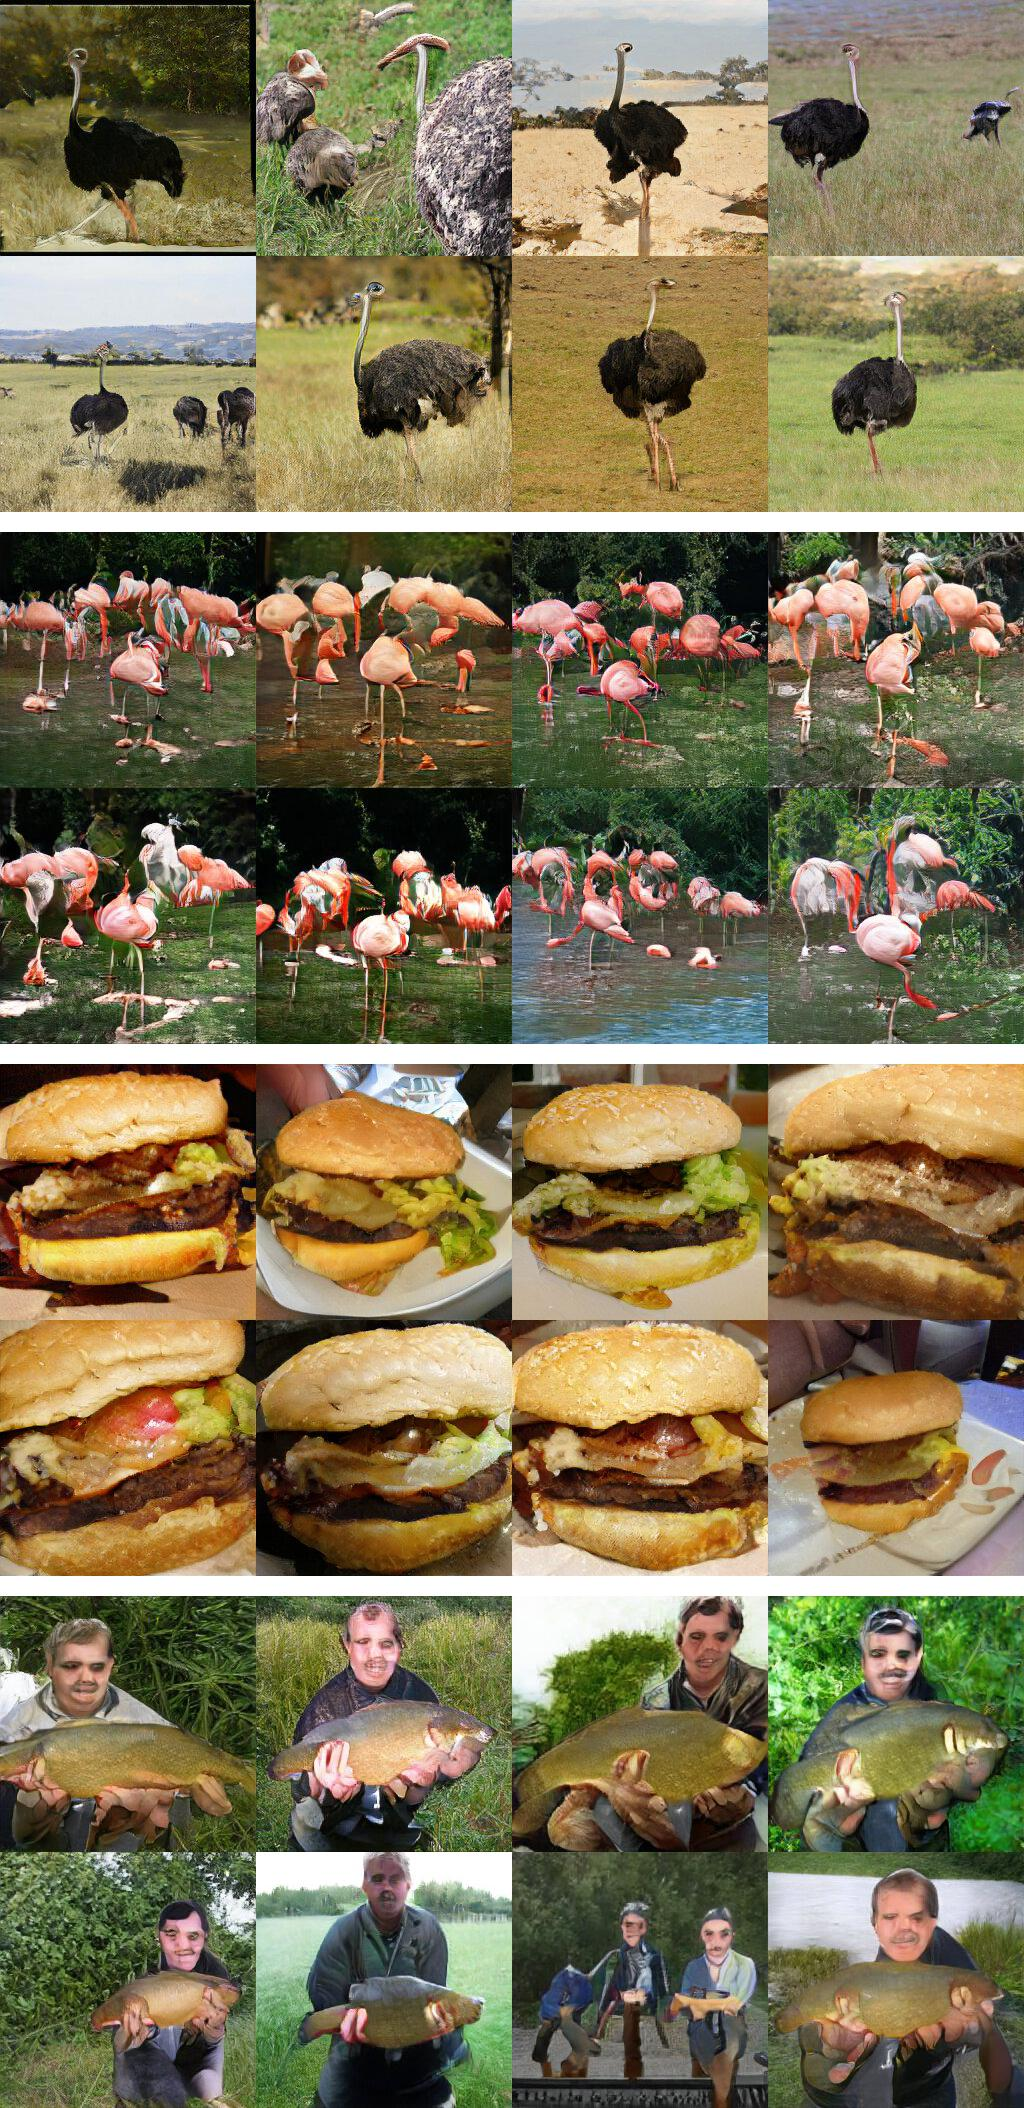
\includegraphics[width=\textwidth]{Images/samples/reflow_biggan-deep-256-t1.jpg}}
    \end{subfigure}\quad
    \begin{subfigure}[]{0.25\textwidth}
    \centerline{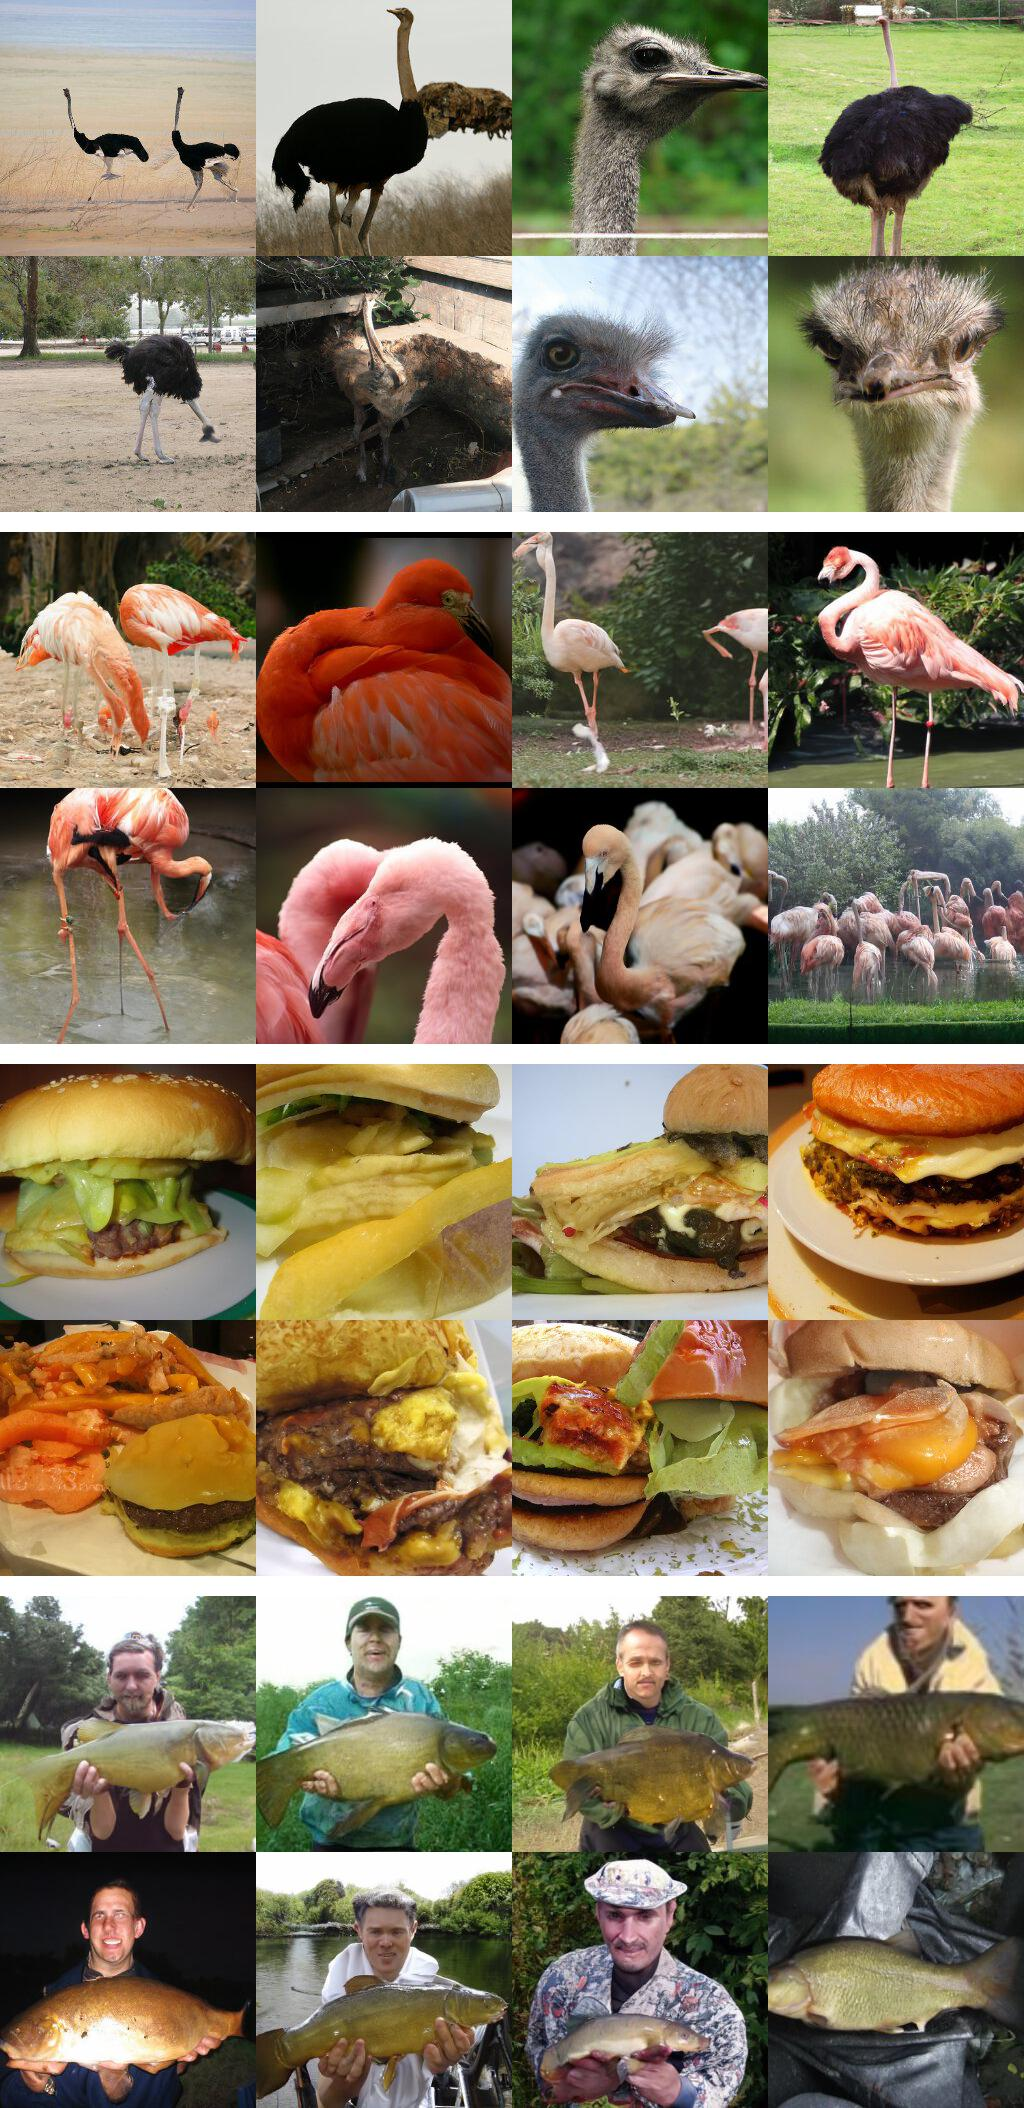
\includegraphics[width=\textwidth]{Images/samples/reflow_imagenet256-guided-250step.jpg}}
    \end{subfigure}\quad
    \begin{subfigure}[]{0.25\textwidth}
    \centerline{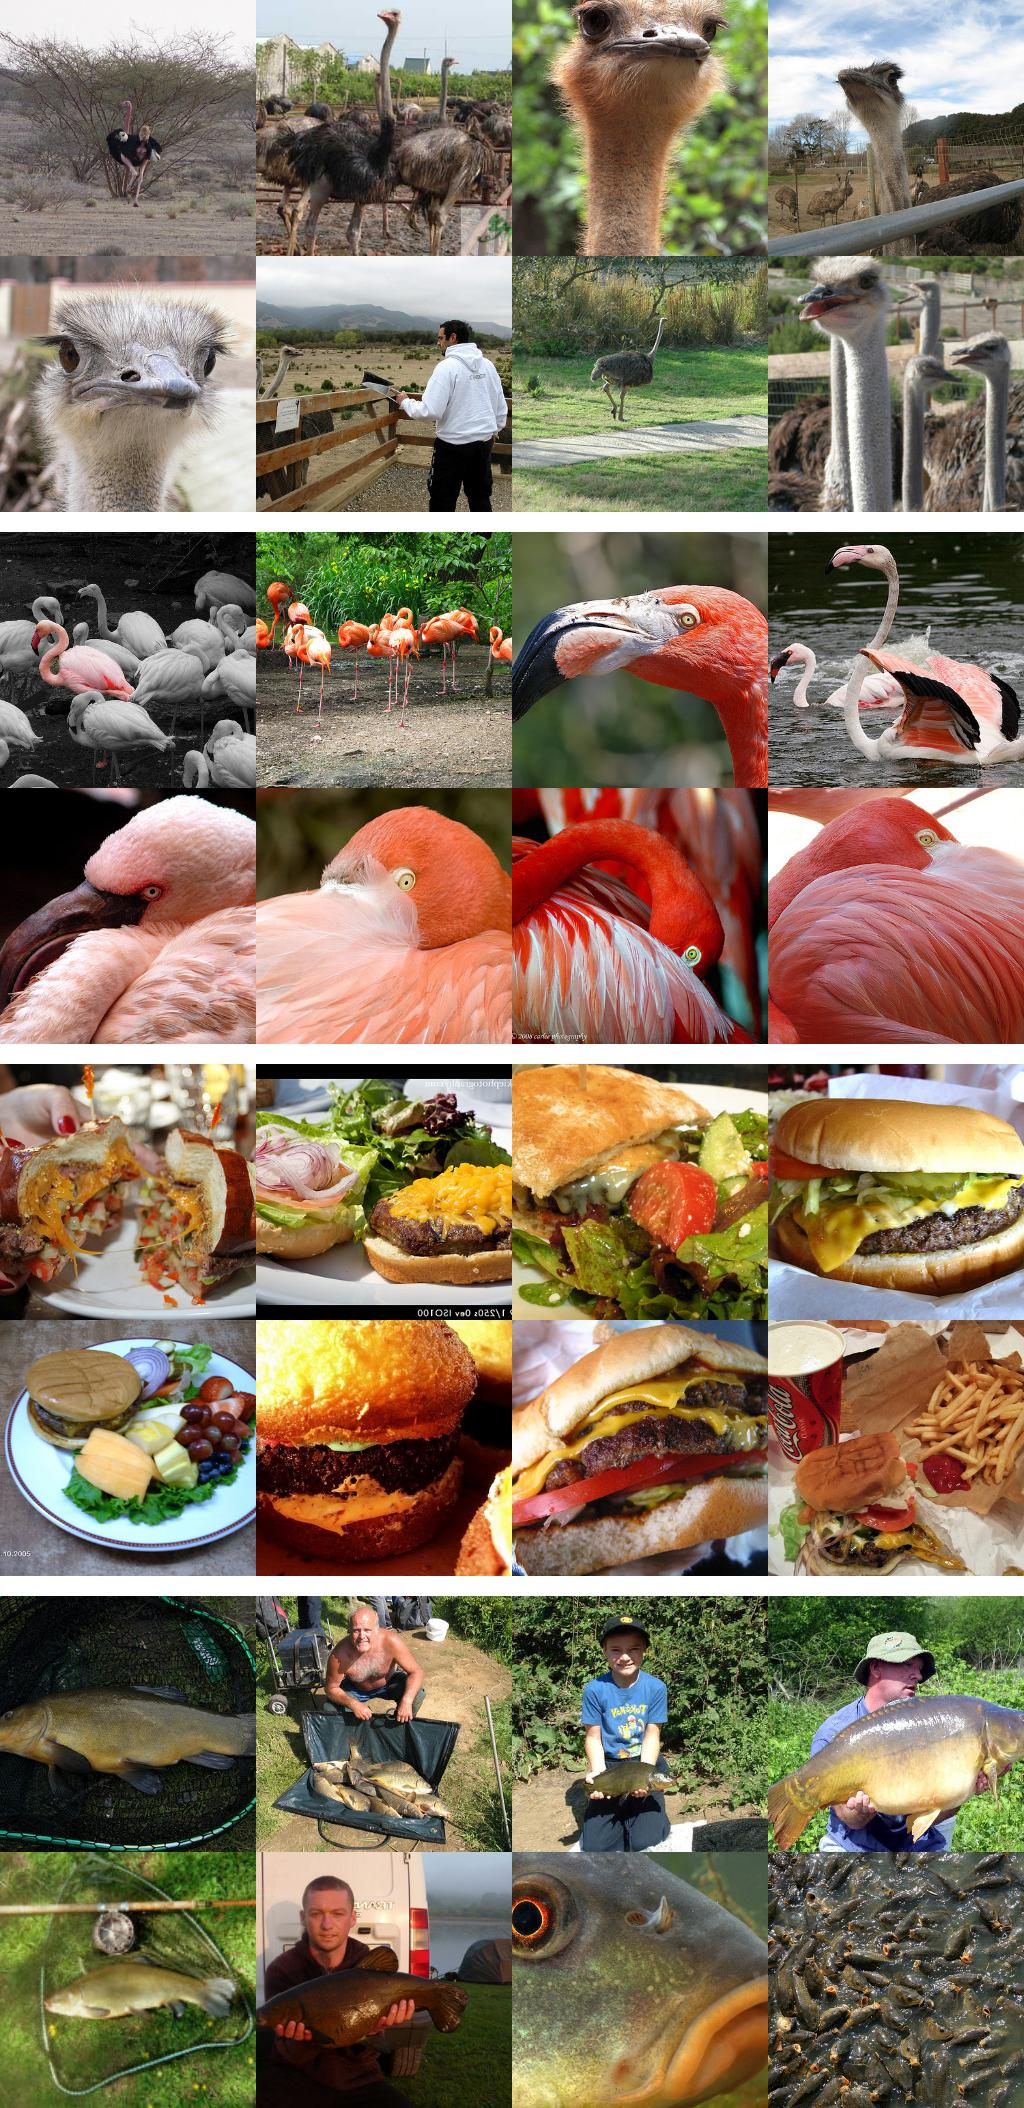
\includegraphics[width=\textwidth]{Images/samples/reflow_real.jpg}}
    \end{subfigure}
    \caption{Vzorci z BigGAN-deep (FID 6.95, levo), v primerjavi z vzorci iz našega modela difuzije z vodenjem (FID 4.59, sredina) in vzorci iz kompleta za treniranje (desno).}
    \label{fig:flamingos}
    \end{center}
    \vskip -0.2in
\end{figure}


% --------------------------------------------- %
% END DM PAGES


% --------------------------------------------- %
% BEGIN DM in HEP PAGES
\newpage
\section{Uporaba difuzijskih modelov v HEP}

Sedaj, ko razumemo difuzijske modele, lahko prikažemo uporabo le-teh za praktično aplikacijo. Osredotočimo se na tri modele, in sicer \caloclouds~\cite{CaloClouds1} in njegovi nadgraditvi \ccedm  ter \cccm  model doslednosti (angl.: \textit{Consistency Model})~\cite{CaloClouds2}. \\

\caloclouds I je strukturiran kot standarden DDPM difuzijski model~\cite{DDPM}. Cilj je bil ustvariti visoko zvestobo predstavitev oblaka točk (angl.: \textit{point cloud}) elektromagnetnih pljuskov v kalorimetrih, ki ponujajo alternativo računalniško dragim pristopom s fiksno strukturo. \ccedm, ki gradi na temeljih, ki jih je postavil \caloclouds I, uvaja več izboljšav. Te temeljijo na Langevinovih modelih dinamičnega ujemanja rezultatov, ki smo jih omenili v prejšnjem poglavju \ref{sec:Diffusion_Models}, manj vrednotenj funkcij modela in uvedbo tehnike destilacije konsistence/doslednosti.

Te spremembe so zasnovane tako, da izboljšajo zvestobo (angl.: \textit{fidelity}) in računalniško učinkovitost simulacijskega procesa ter izpolnjujejo zahteve eksperimentov, kot sta bodoči mednarodni veliki detektor (ILD~\cite{ILD}) in veliki hadronski trkalnik z visoko svetilnostjo (HL-LHC~\cite{HL-LHC}). \\

Modela sta bila ovrednotena na podlagi zmožnosti natančne simulacije različnih fizikalnih lastnosti elektromagnetnih pljuskov v kalorimetričnih detektorjih (kot opisano v poglavju \ref{sec:Geant4}). Te lastnosti vključujejo porazdelitev energije na celico, radialne in vzdolžne profile pljuskov, izračune težišča, porazdelitev vidne energije in število zadetkov nad pragom. Primerjalne analize s \geant, ki nam predstavlja simulacije temeljnih resnic, so pokazale, da čeprav oba modela izkazujeta visoko zvestobo pri predstavljanju teh fizikalnih lastnosti, je \ccedm  na splošno boljši od predhodnika, zlasti v smislu rezultatov zvestobe, ki temeljijo na Wassersteinovi metriki razdalje\footnote{Wasserstein metrika je funkcija razdalje, definirana med verjetnostnimi porazdelitvami na danem metričnem prostoru $M$~\cite{Wasserstein}.}.



\subsection{Fizikalna uspešnost} 
\label{sec:Results_Physics}

Primerjamo različne porazdelitve kalorimetrskih pljuskov iz ref.~\cite{CaloClouds1} med testnim nizom \geant in nizi podatkov, ustvarjenimi z uporabo vseh treh modelov. Najprej primerjamo različne opazovane vrednosti na ravni celic in pljuske, ki so izračunani iz modela ustvarjenih pljuskov, s simulacijami \geant z vzorci vpadnih fotonov z energijami, enakomerno porazdeljenimi med 10 in 90 GeV (imenovani tudi polni spekter). Na sliki \ref{fig:Ehits_Radial_Spinal} raziskujemo tri predstavitve energije, porazdeljene v celicah kalorimetra. Porazdelitev energije na celico vsebuje energijo celic vseh pljuskov v testnem nizu podatkov. Vsi modeli razmeroma dobro opisujejo porazdelitev celične energije.

\begin{figure*}[htb!]
    \centering
    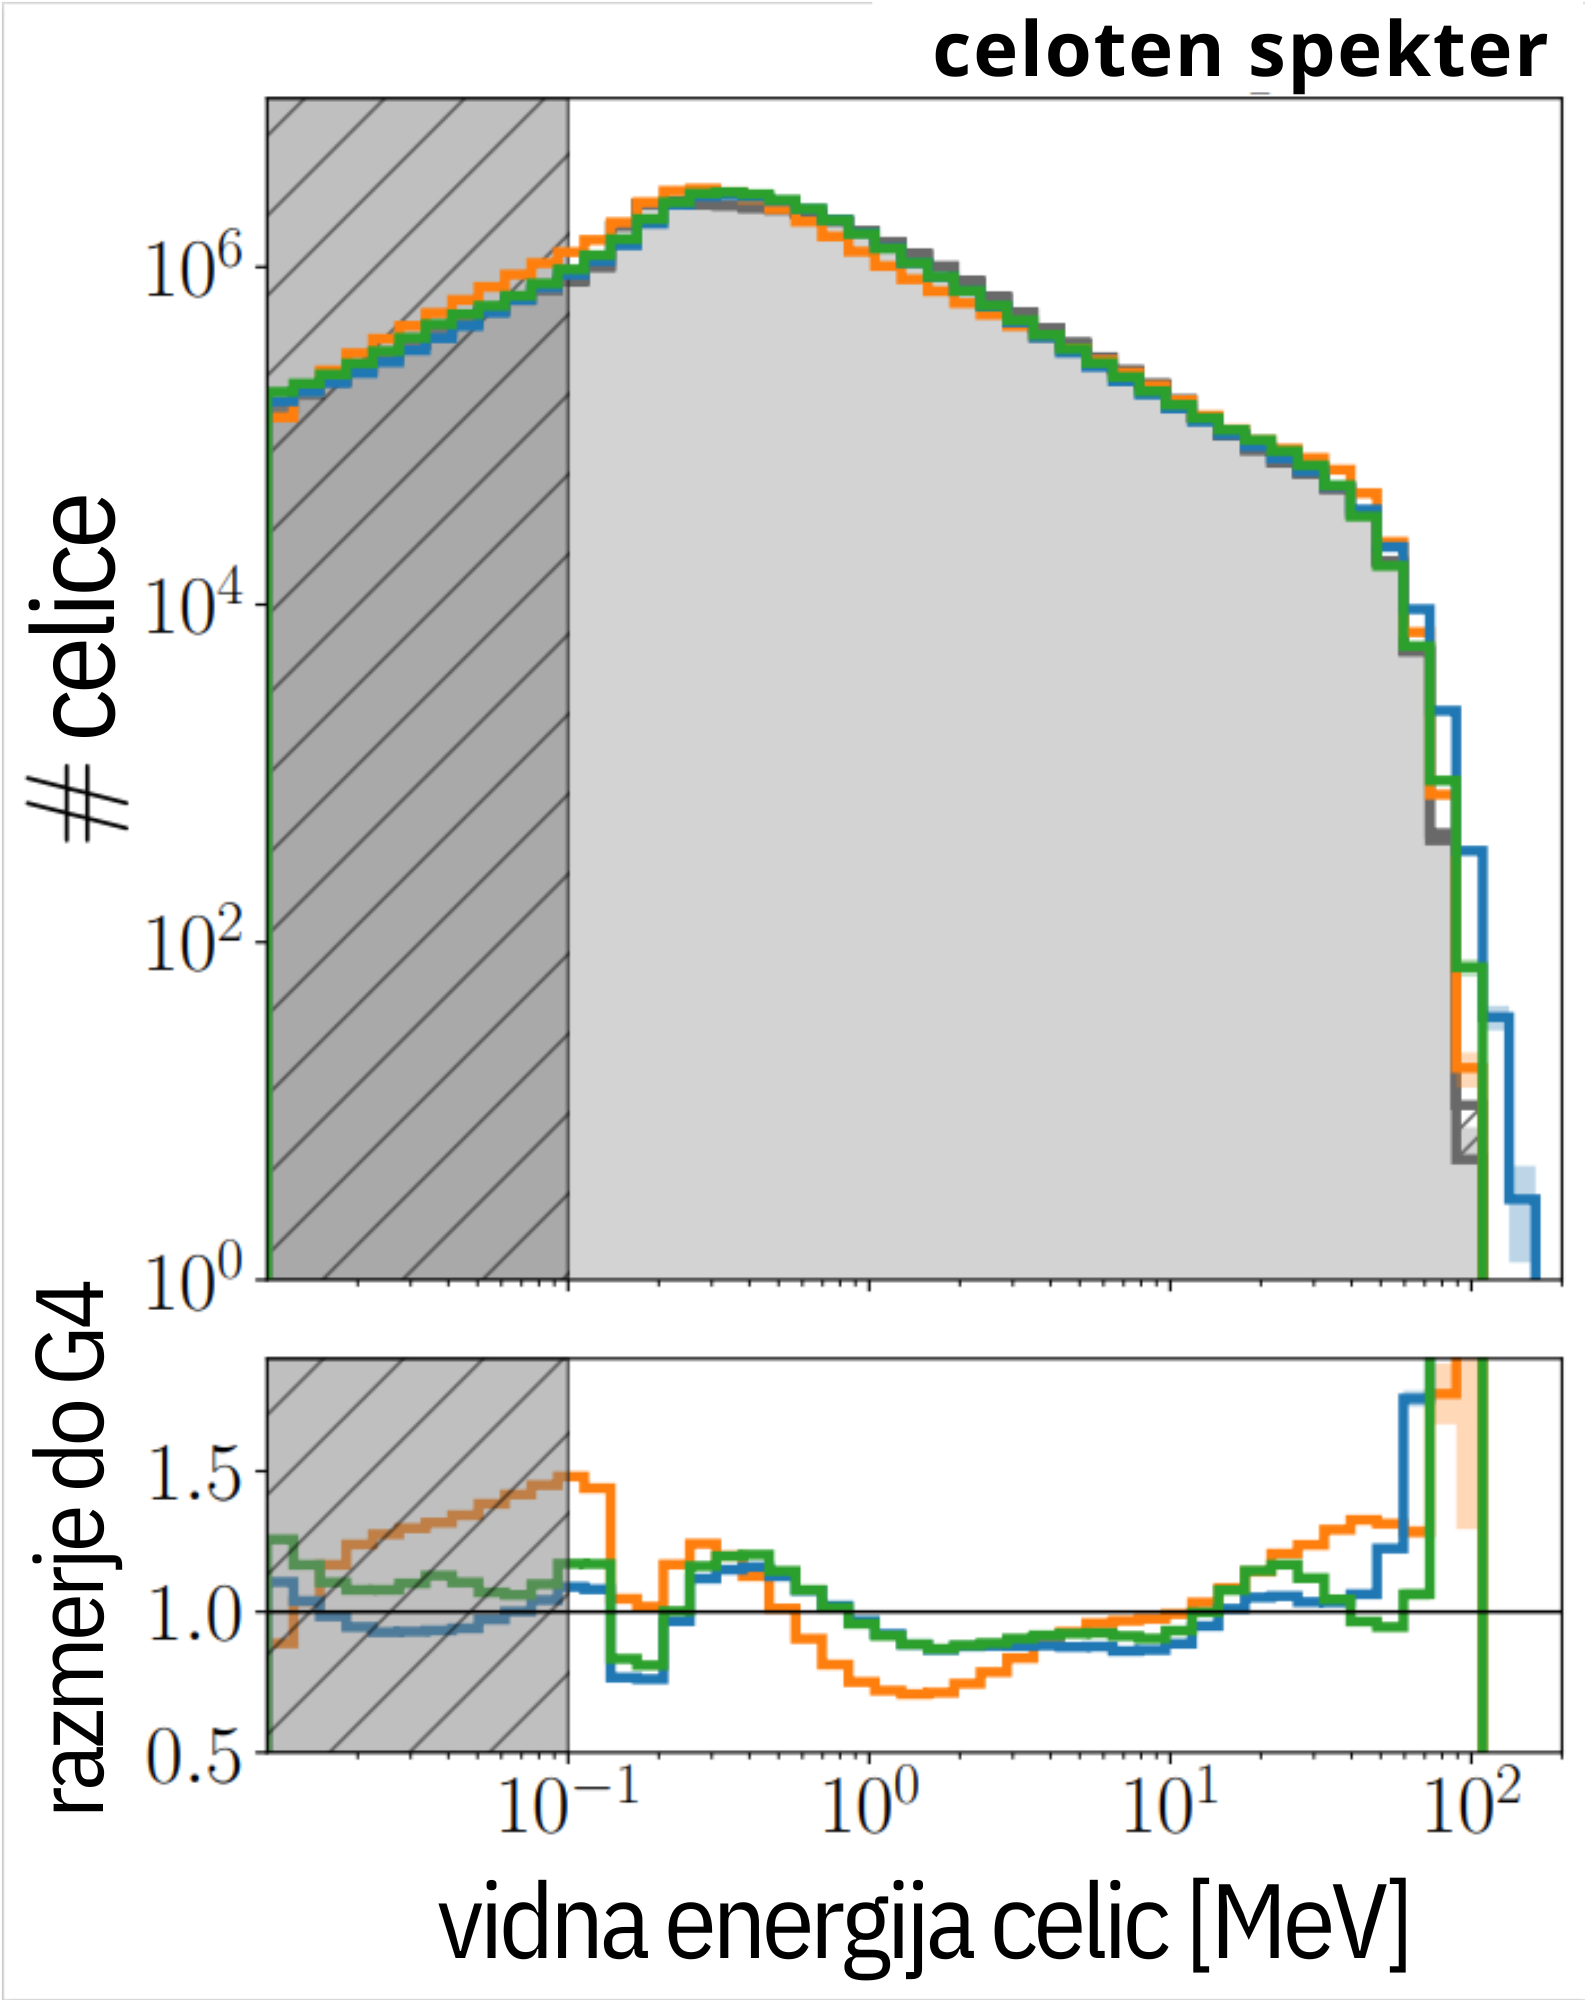
\includegraphics[width=0.30\textwidth]{Images_SLO/hits_SLO.png}
    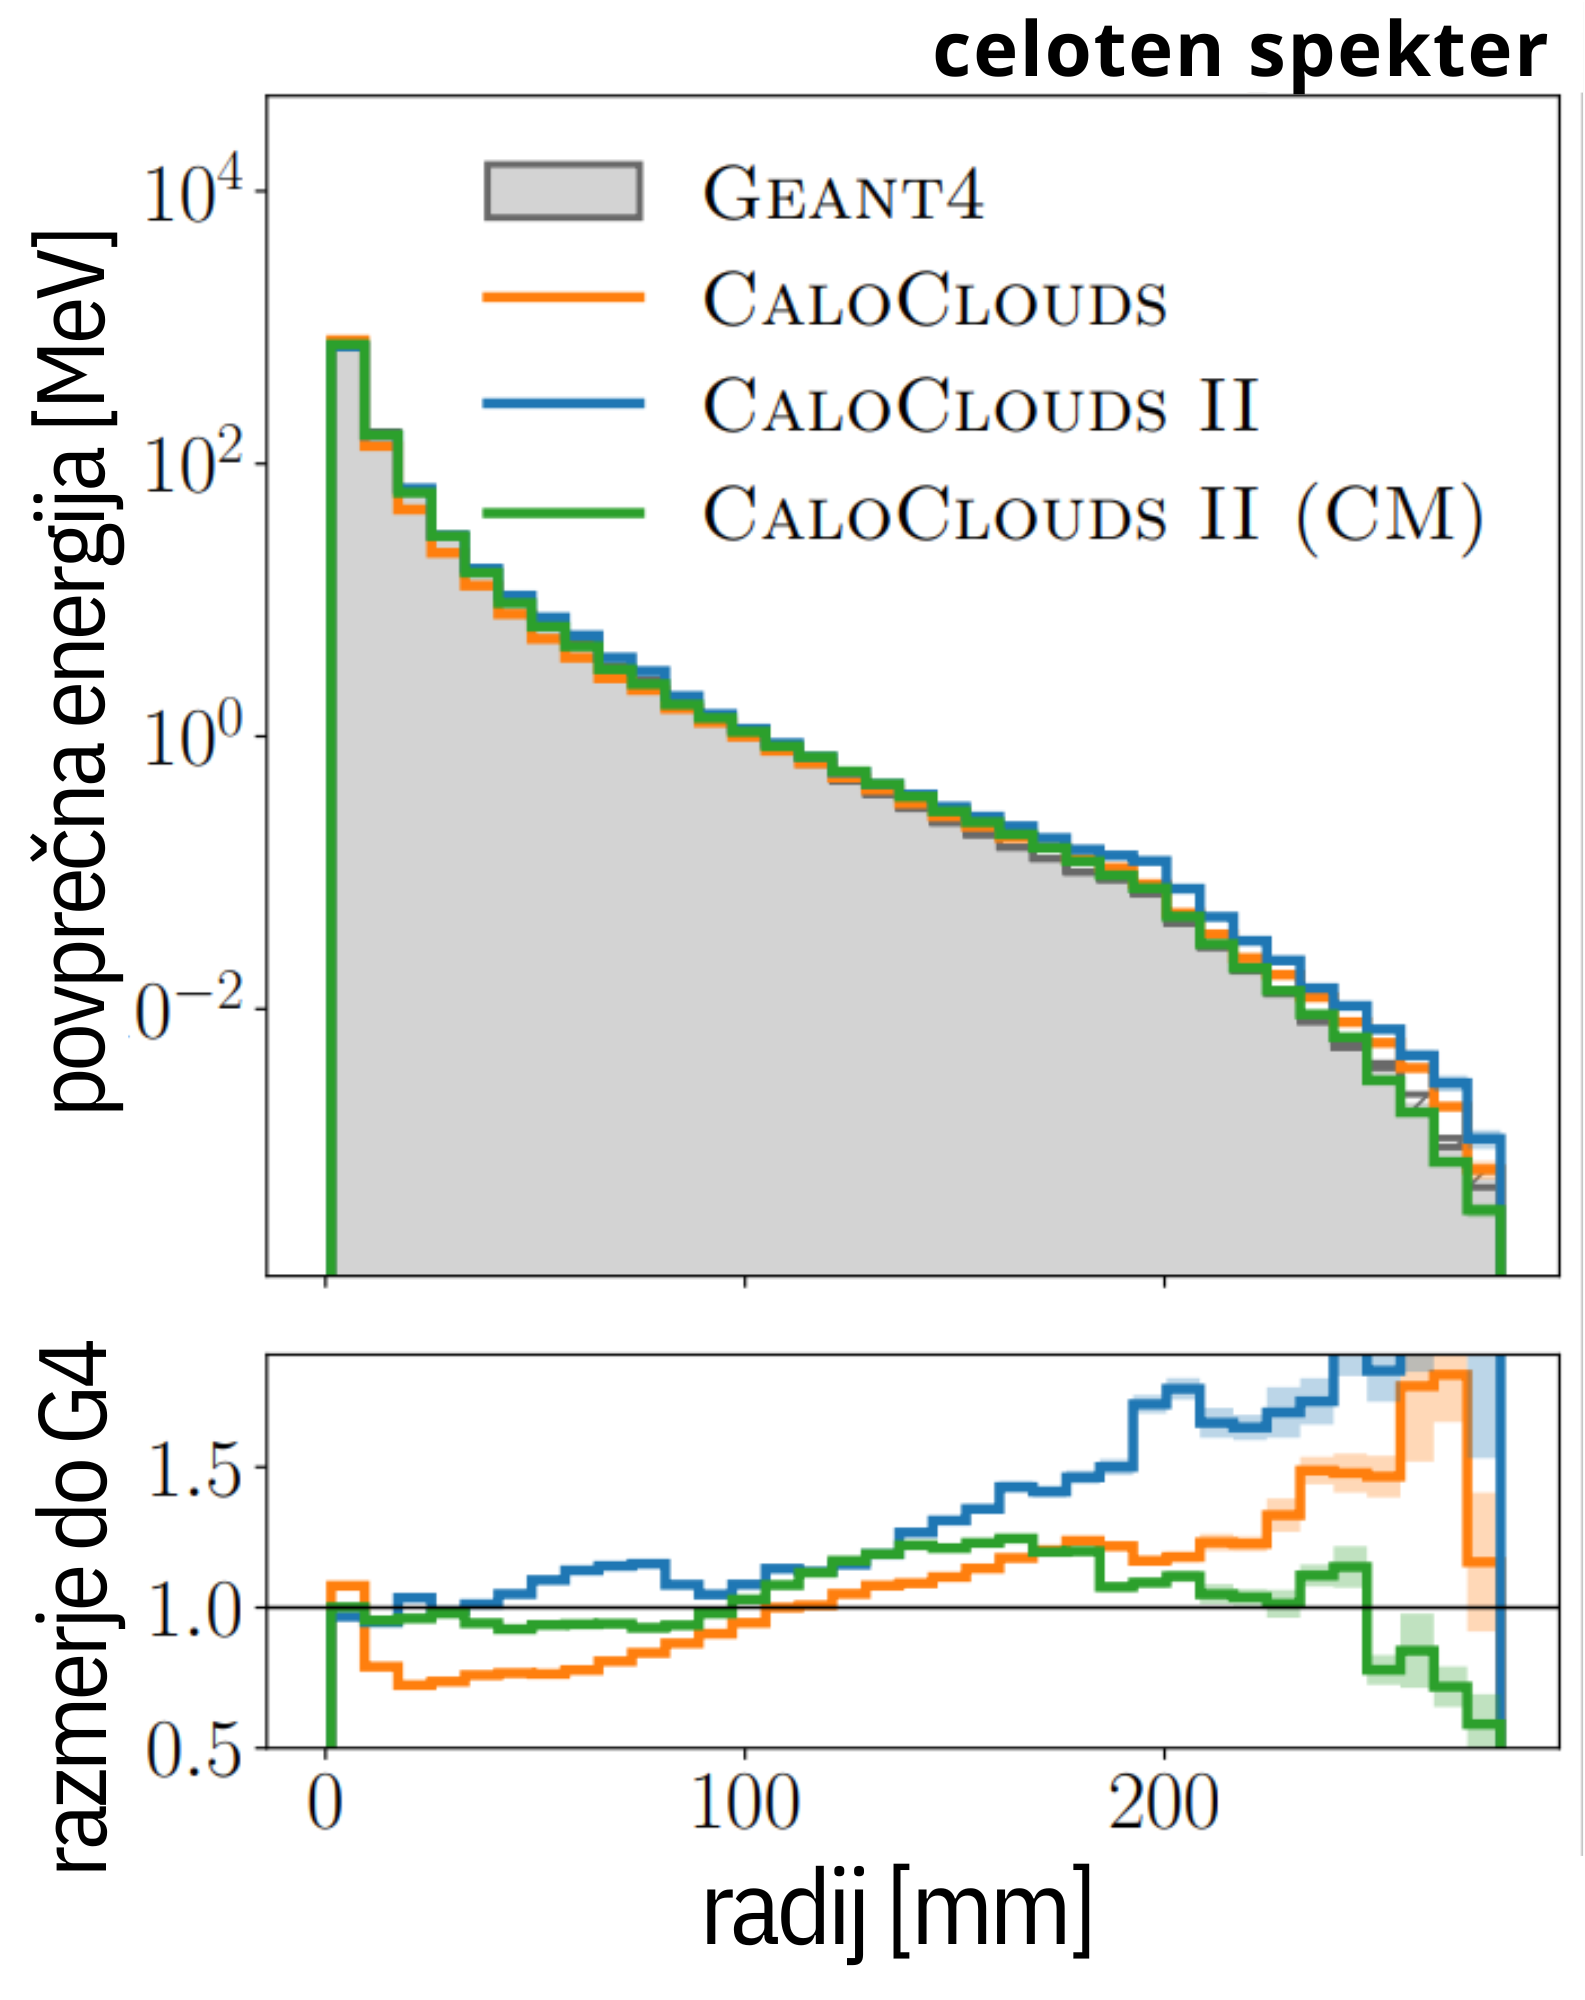
\includegraphics[width=0.30\textwidth]{Images_SLO/radial_SLO.png}
    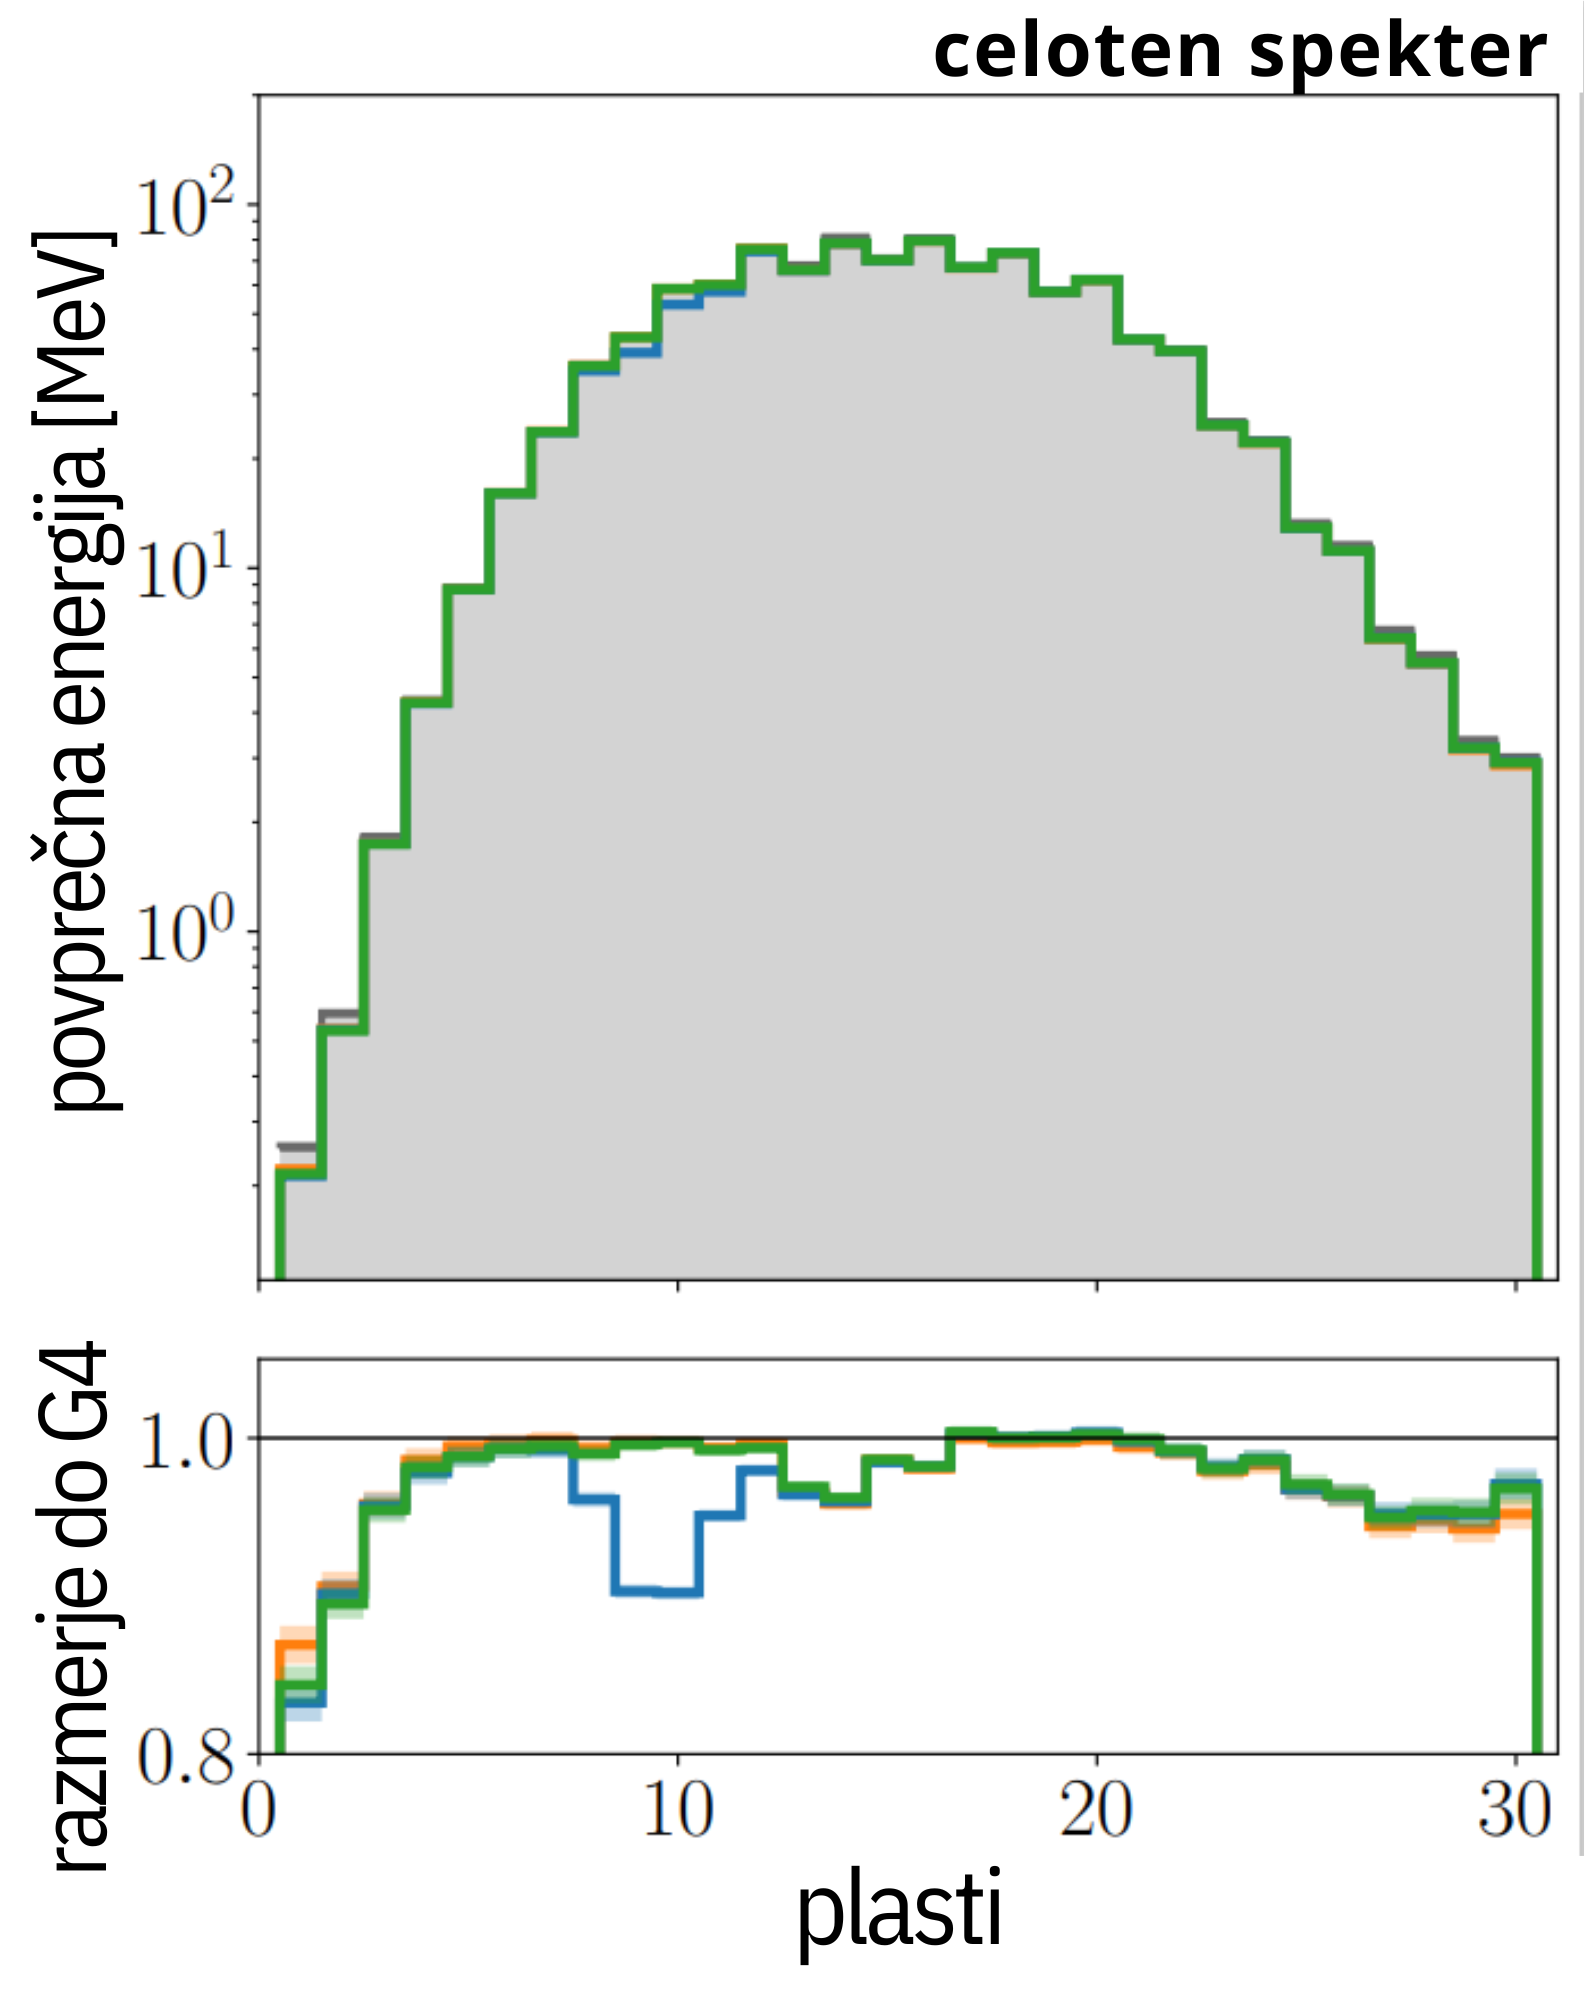
\includegraphics[width=0.30\textwidth]{Images_SLO/spinal_SLO.png}
    \caption{Histogram celične porazdelitve energije (levo), profila radialnega (na sredini) in vzdolžnega profila pljuskov (desno) za \geant, \caloclouds, \ccedm, in \cccm.}
    \label{fig:Ehits_Radial_Spinal}
    %\hspace{0.5cm}
\end{figure*}

%\begin{figure*}[htb!]
%    \centering
%    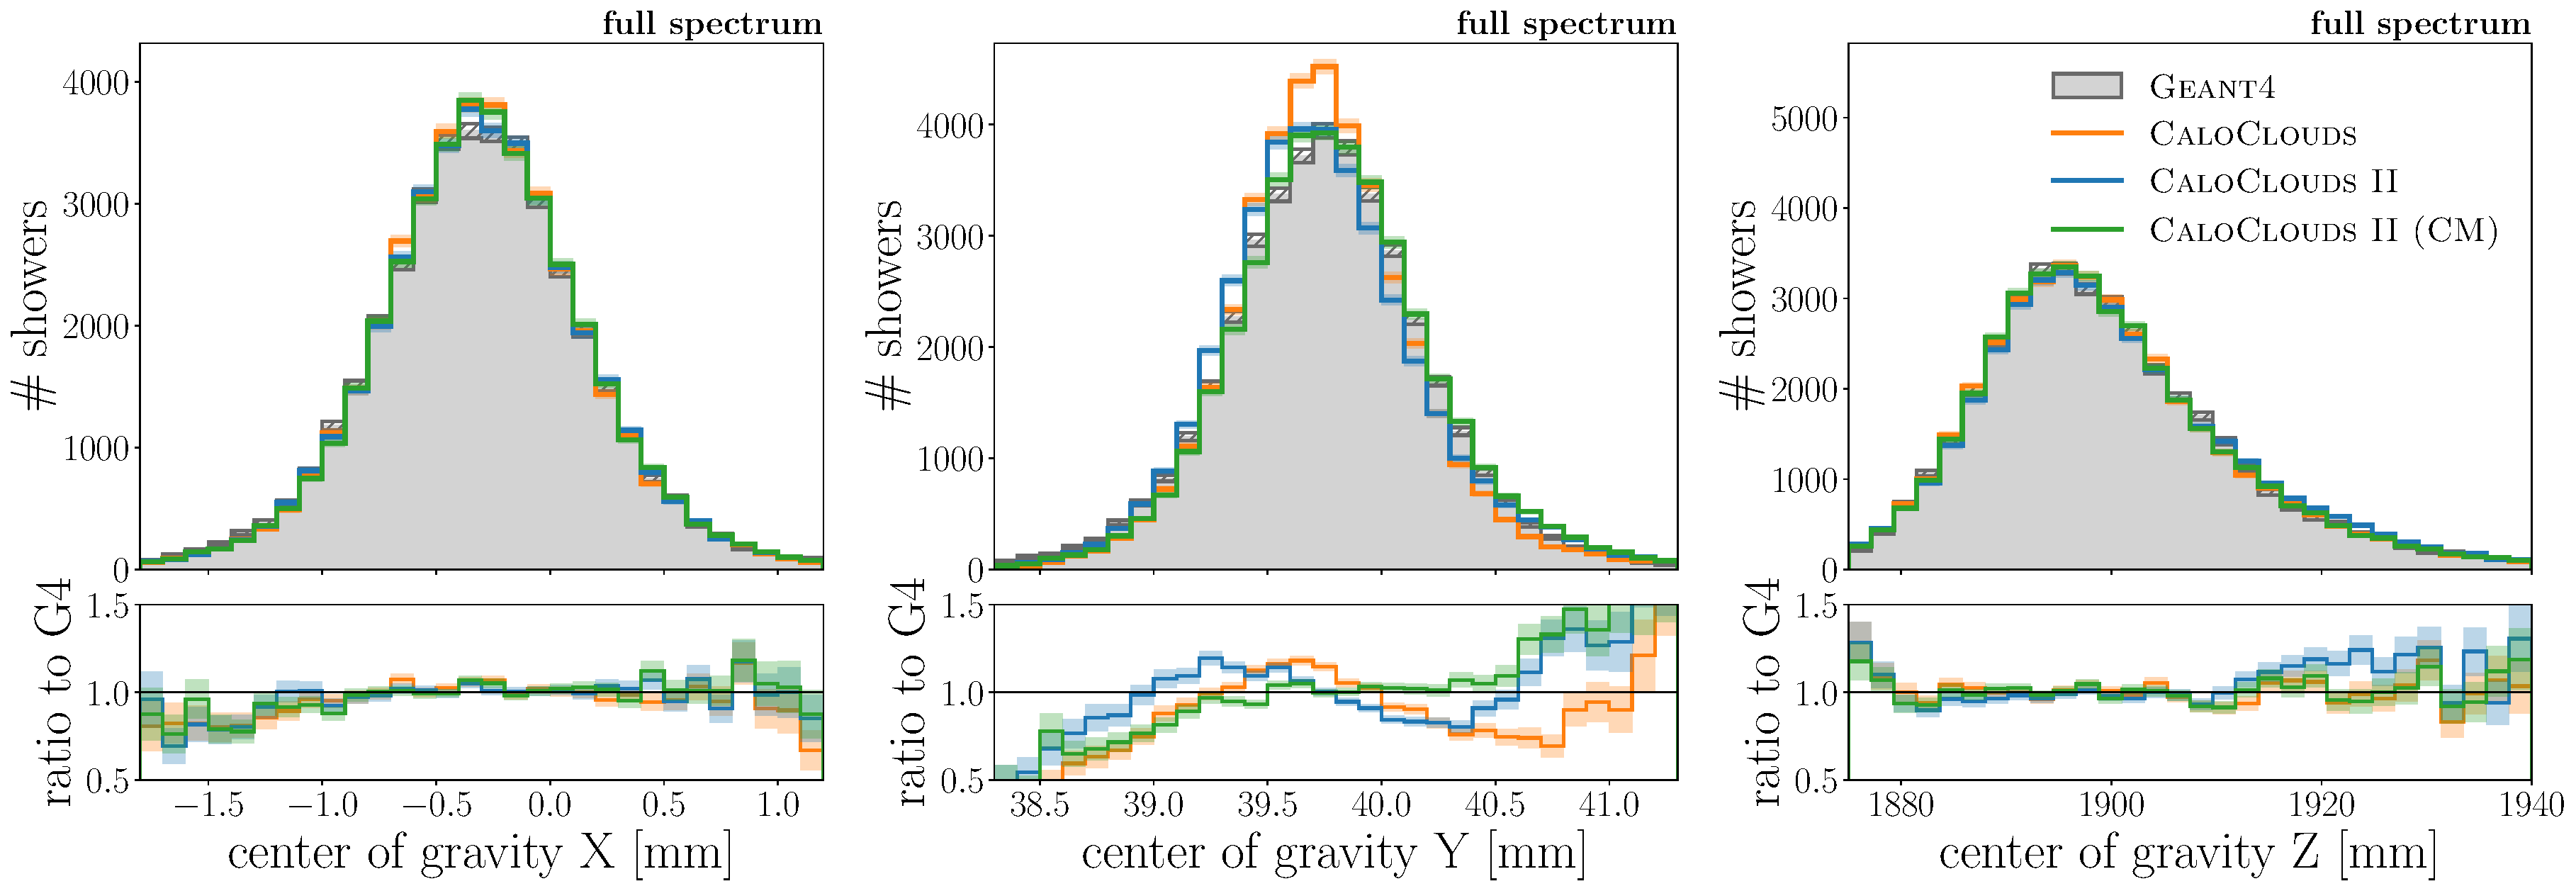
\includegraphics[width=1\textwidth]{Images/samples/cog.pdf}
%    \caption{
%    Position of the center of gravity of showers along the $X$ (left), $Y$ (center), and $Z$ (right) directions. All distributions are calculated for 40,000 showers with a uniform distribution of incident particle energies between 10 and 90~GeV.
%    The error band corresponds to the statistical uncertainty in each bin.
%    }
%    \label{fig:CoG}
%    \hspace{0.5cm}
%\end{figure*}

Nato raziščemo zanesljivost modelov za energije posameznega vpadnega fotona 10, 50 in 90 GeV \ref{fig:Esum_Occ}. Skupna energija je dobro zastopana pri vseh treh modelih. Število zadetkov je ena najtežjih porazdelitev za generativni model oblaka točk. Tukaj je visoka zvestoba še vedno dosežena z uporabo kalibracije števila točk~\cite{CaloClouds2}.

\begin{figure*}[htb!]
    \centering
   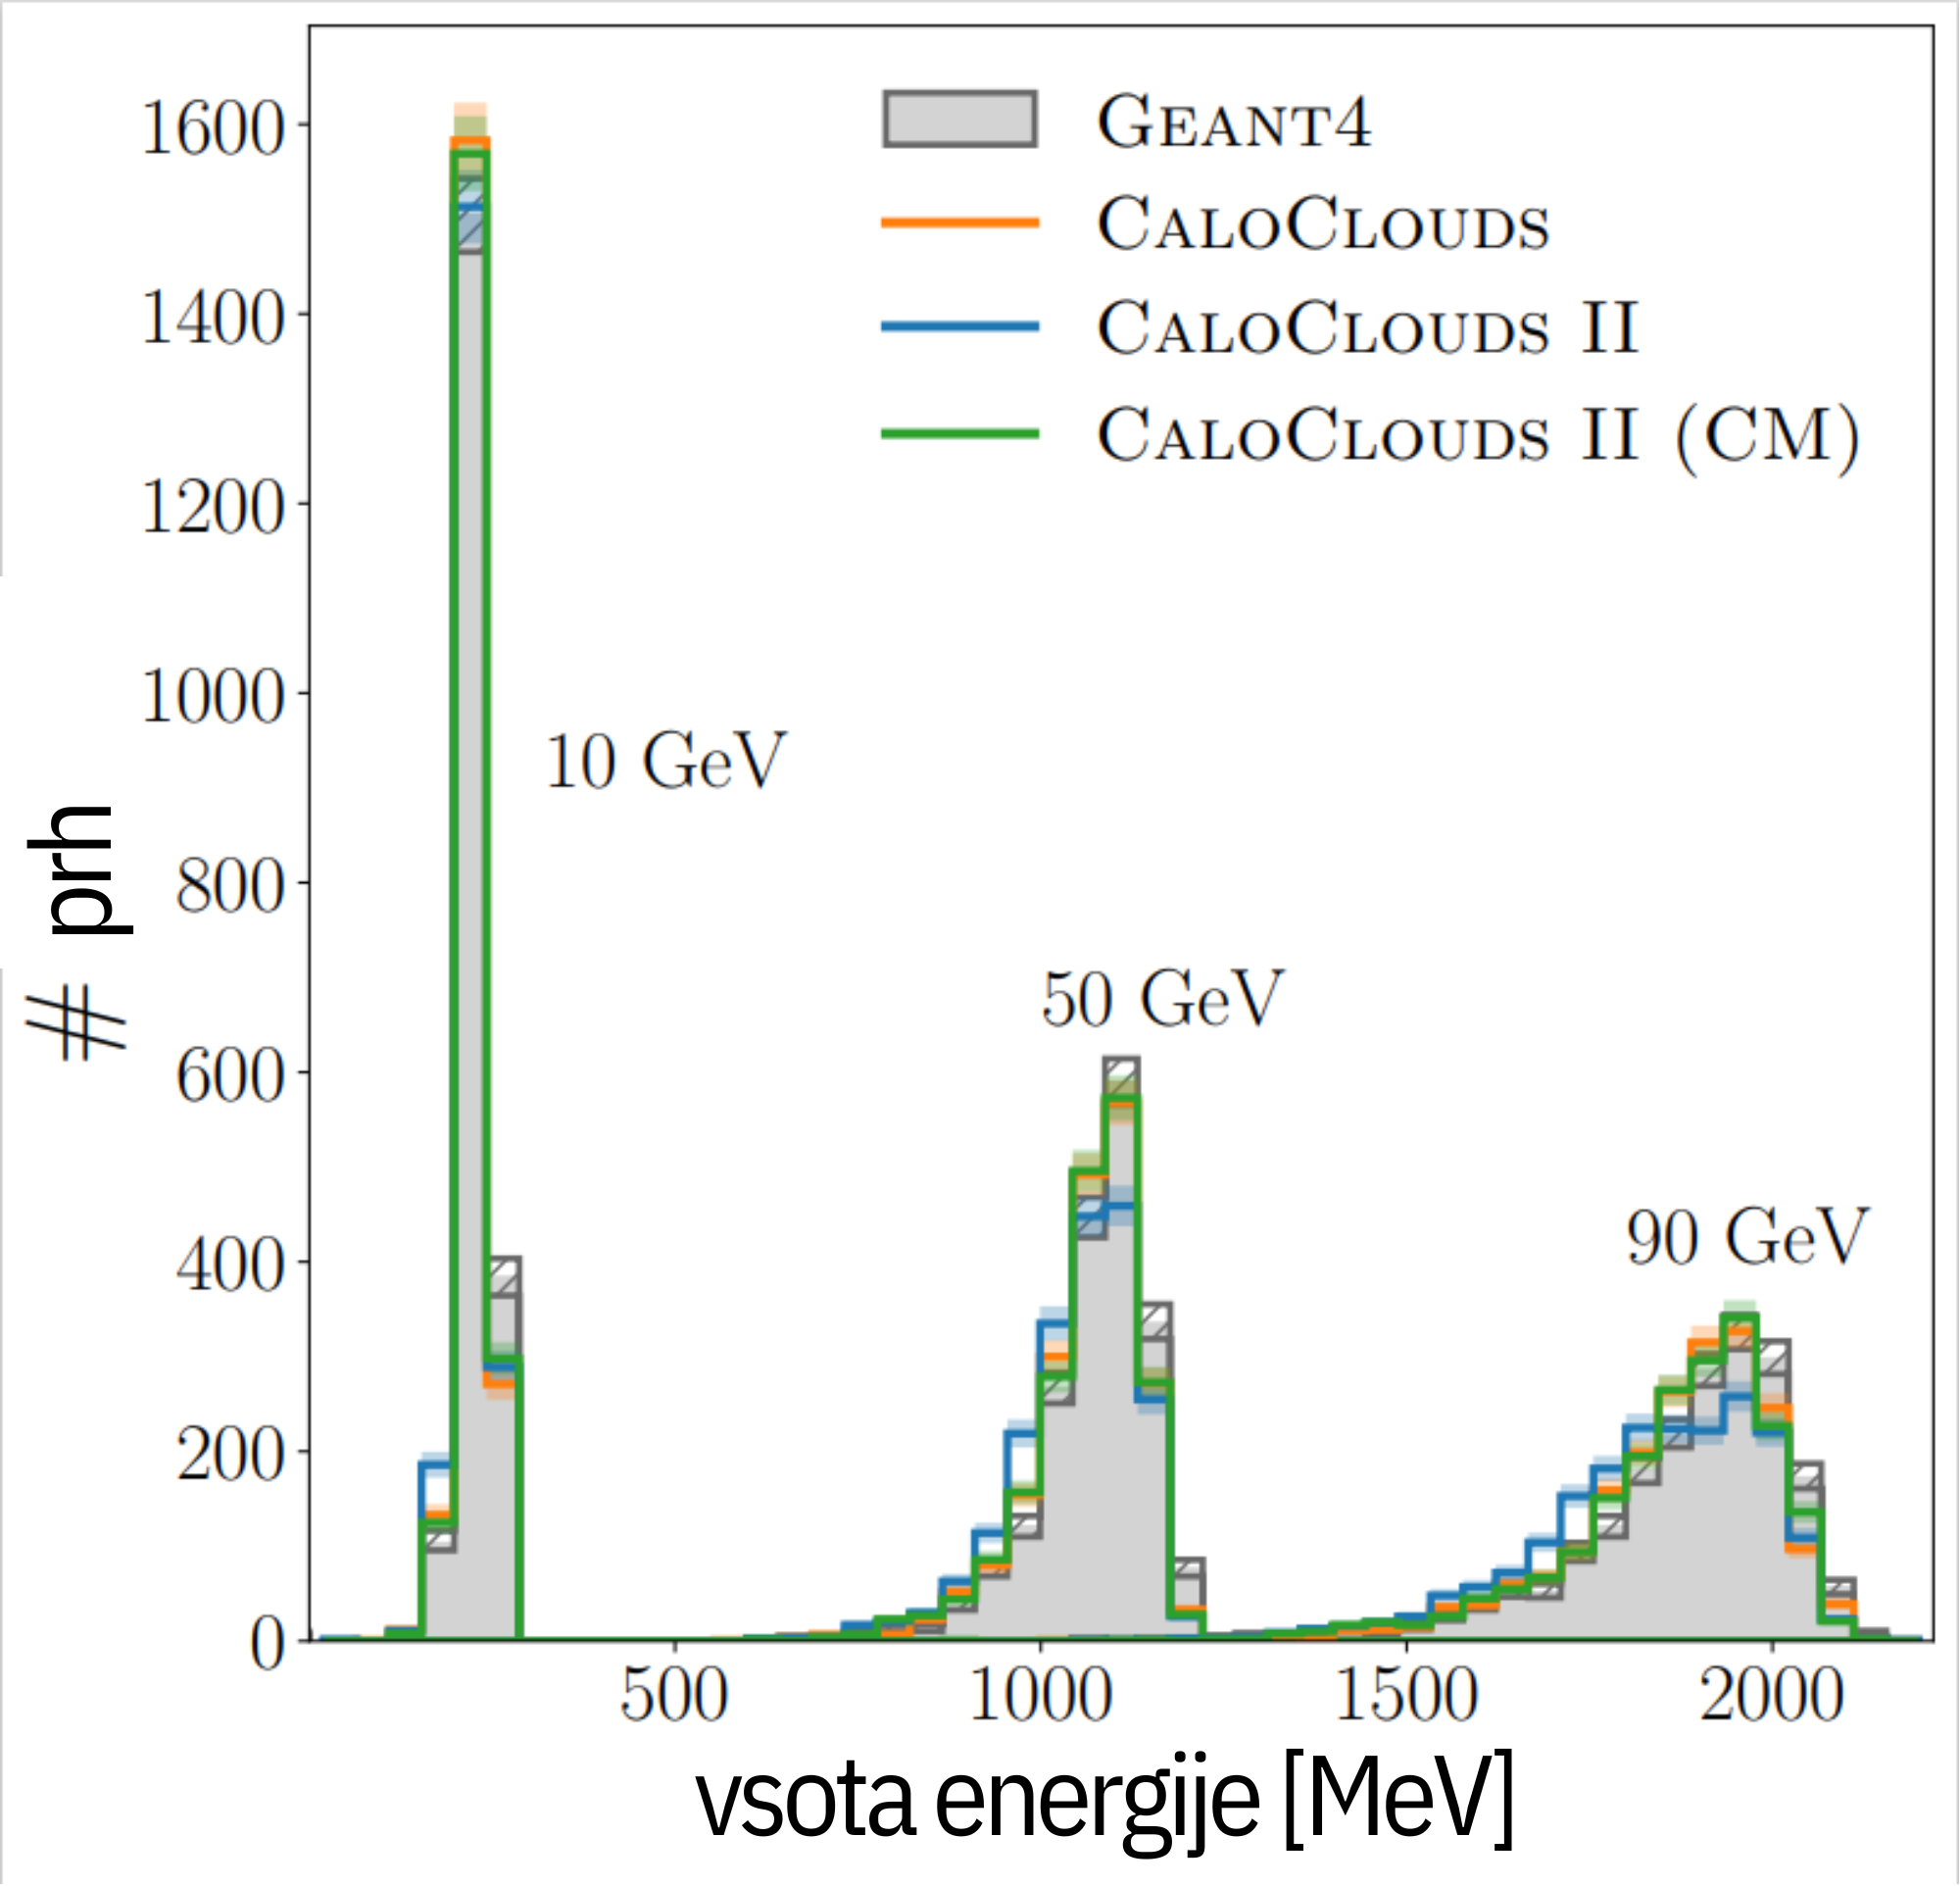
\includegraphics[width=0.41\textwidth]{Images_SLO/e_sum_singleE _SLO.pdf.png}
    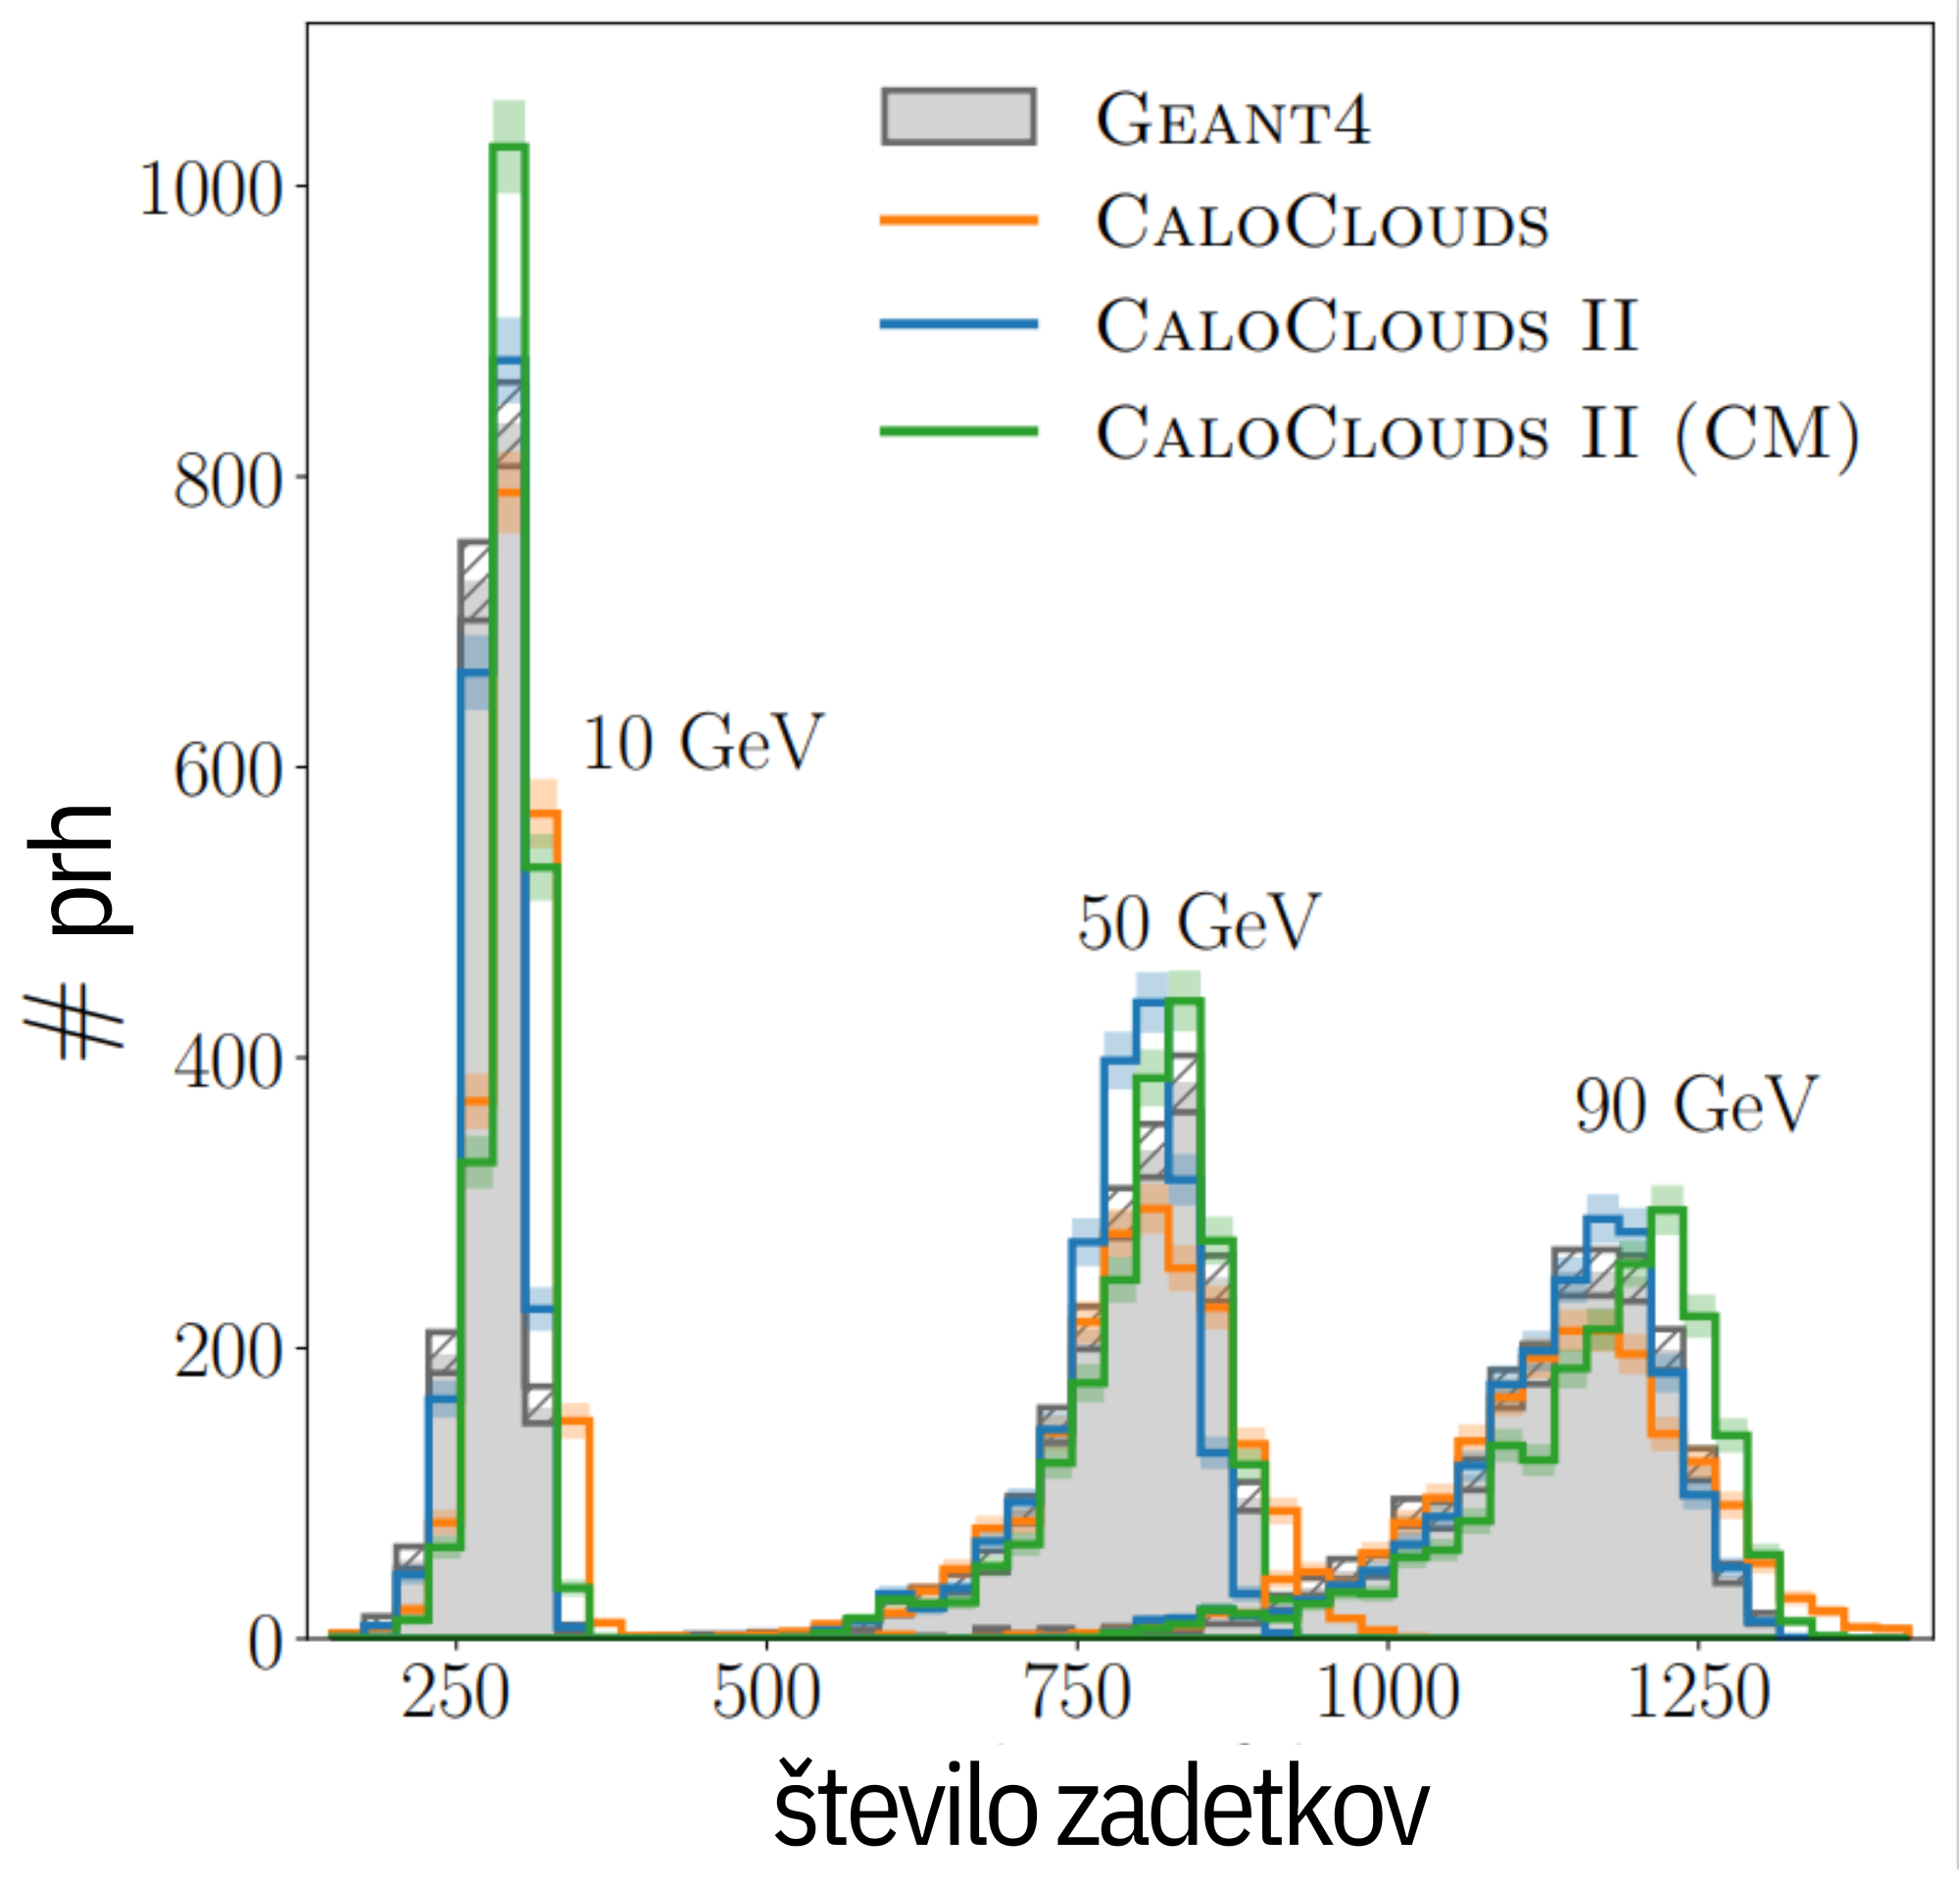
\includegraphics[width=0.41\textwidth]{Images_SLO/occ_singleE _SLO.pdf.png}
    \caption{
    Vidna porazdelitev vsote energije (levo) in števila zadetkov (celice z deponirano energijo nad polovico praga) (desno) za plohe pri 10, 50 in 90 GeV. Za vsako energijo in model je prikazanih 2000 pljuskov. Pas napake ustreza statistični negotovosti v vsakem intervalu (angl.: \textit{bin}).
    }
    \label{fig:Esum_Occ}
    \hspace{0.5cm}
\end{figure*}


%\newpage
\subsection{Evalvacijski rezultati}
\label{sec:Results_Evaluation}

V tabeli \ref{table:wasserstein_scores} je predstavljena primerjava uspešnosti modelov z rezultati na podlagi 1-Wasserstein razdalje za različne standardizirane opazovalke pljuskov. Predstavljene vrednosti so povprečje in standardna deviacija 10 izračunanih rezultatov, ki primerjajo 50k \geant  in 50k ustvarjenih pljuskov, ref.~\cite{CaloClouds2}.

\begin{table*}[htb!]
\sisetup{
separate-uncertainty=true,
table-format=4.3(5)
}
\centering
%\vspace{15pt}
\resizebox{\textwidth}{!}{
\begin{tabular}{lcccccccc}
\toprule
Simulator & $W_1^{N_\mathrm{hits}}$ & $W_1^{E_\mathrm{vis}/E_\mathrm{inc}}$ & $W_1^{E_\mathrm{cell}}$ & $W_1^{E_\mathrm{long}}$ & $W_1^{E_\mathrm{radial}}$ & $W_1^{m_{1,X}}$ & $W_1^{m_{1,Y}}$ & $W_1^{m_{1,Z}}$ \\
          & $(\times 10^{-3})$      & $(\times 10^{-3})$             & $(\times 10^{-3})$      & $(\times 10^{-3})$       & $(\times 10^{-3})$        & $(\times 10^{-3})$     & $(\times 10^{-3})$     & $(\times 10^{-3})$     \\
\midrule
\geant      & 0.7 $\pm$ 0.2         & 0.8 $\pm$ 0.2                  & 0.9 $\pm$ 0.4           & 0.7 $\pm$ 0.8            & 0.7 $\pm$ 0.1            & 0.9 $\pm$ 0.1          & 1.1 $\pm$ 0.3          & 0.9 $\pm$ 0.3   \\
            & & &\\
\caloclouds & \textbf{2.5 $\pm$ 0.3}& 11.4 $\pm$ 0.4                 & 15.9 $\pm$ 0.7          & \textbf{2.0 $\pm$ 1.3}   & 38.8 $\pm$ 1.4            & 4.0 $\pm$ 0.4          & 8.7 $\pm$ 0.3          & 1.4 $\pm$ 0.5 \\
\ccedm      & 3.6 $\pm$ 0.5         & 26.4 $\pm$ 0.4                 & \textbf{15.3 $\pm$ 0.6} & 3.7 $\pm$ 1.6            & 11.6 $\pm$ 1.5            & \textbf{2.4 $\pm$ 0.4} & \textbf{7.6 $\pm$ 0.2} & 3.9 $\pm$ 0.4          \\
\cccm       & 6.1 $\pm$ 0.7         & \textbf{9.8 $\pm$ 0.5}         & 16.0 $\pm$ 0.7          & \textbf{2.0 $\pm$ 1.4}   & \textbf{8.3 $\pm$ 1.9}    & 3.0 $\pm$ 0.4          & 9.5 $\pm$ 0.6          & \textbf{1.2 $\pm$ 0.5} \\
\bottomrule 
\end{tabular}
}
%\vspace{15pt}
\caption{Primerjava uspešnosti modelov na podlaki Wassersteinove razdalje.}
\label{table:wasserstein_scores}
\end{table*}


\subsection{Časovna razporeditev}
\label{sec:Results_Timings}

V tem razdelku primerjamo povprečni čas za izdelavo enega samega kalorimetrsk\-ega pljuska in raziskujemo pospešitev glede na osnovno simulacijo \geant. Tako na enem samem procesorju kot na grafičnem procesorju NVIDIA\textsuperscript{\tiny\textregistered} A100 so ustvarili $25\times2000$ pljuskov z enako enakomerno porazdelitvijo energije med 10 in 90 GeV. Zlasti časovni razpored na enem CPU je zanimiv za trenutne aplikacije generativnih modelov v HEP, saj so CPU veliko bolj dostopni kot GPU in trenutna računalniška infrastruktura temelji na simulacijah, ki se izvajajo na CPU. Rezultati časovnega merjenja so predstavljeni v tabeli \ref{table:timing}. Upoštevajte, da \geant trenutno ni združljiv z grafičnimi procesorji in da so grafični procesorji bistveno dražji od procesorjev.
Kljub temu opazimo drastično izboljšavo hitrosti proizvodnje simulacij, \cccm je kar $46\times$ hitrejši na CPU in $1873\times$ hitrejši z uporabo GPU.


\begin{table*}[htb!]
\sisetup{
separate-uncertainty=true,
table-format=4.3(5)
}
\centering
%\vspace{15pt}
\resizebox{\textwidth}{!}{
\begin{tabular}{llcc|cr}
\toprule
Strojna Oprema & Simulator & NFE & Velikost Serije & {Čas / Prha [ms]} & Pospešitev \\
\midrule
CPU & \geant & & & 3914.80 $\pm$ 74.09 & $\times 1$ \\
    & & &\\
    & \caloclouds & 100 & 1 & 3146.71 $\pm$ 31.66 & $\times 1.2$ \\   %
    & \ccedm & 25 & 1 & 651.68 $\pm$ 4.21 & $\times 6.0$ \\    %
    & \cccm & 1 & 1 & 84.35 $\pm$ 0.22 & $\times 46$ \\  %
    & & &\\
GPU & \caloclouds & 100 & 64 & 24.91 $\pm$ 0.72 & $\times 157$ \\  %
    & \ccedm & 25 & 64 & 6.12 $\pm$ 0.13 & $\times 640$ \\  %
    & \cccm & 1 & 64 & 2.09 $\pm$ 0.13 & $\times 1873$ \\  %
\bottomrule 
\end{tabular}
}
%\vspace{15pt}
    %\caption{Comparison of the computational    performance of \caloclouds, \ccedm, and \cccm to the baseline \geant simulator on a single core of an Intel\textsuperscript{\tiny\textregistered} Xeon\textsuperscript{\tiny\textregistered} CPU E5-2640 v4 (CPU) and on an NVIDIA\textsuperscript{\tiny\textregistered} A100 with 40~GB of memory (GPU). 2,000 showers were generated with incident energy uniformly distributed between 10 and 90~GeV. Values presented are the means and standard deviations over 10 runs. The number of function evaluations (NFE) indicate the number of diffusion model passes.}
    \caption{Primerjava računalniške zmogljivosti vseh 3 modelov.}
\label{table:timing}
\end{table*}

% --------------------------------------------- %
% END DM in HEP PAGES


% --------------------------------------------- %
% BEGIN CONCLUSION PAGE
%\newpage
\section{Zaključek}

Skratka, uporaba generativnih modelov umetne inteligence, kot je \caloclouds, predstavlja pomemben napredek pri simulaciji zapletenih fizikalnih pojavov, kot je pljuskanje delcev v detektorjih, kot sta mednarodni veliki detektor (ILD) in veliki hadronski trkalnik visoke svetilnosti (HL-LHC). 
Ti modeli ponujajo obetavne poti za pospeševanje simulacij in s tem omogočajo nova odkritja v temeljni fiziki. Poleg tega, onkraj akademskega sveta in industrije obstaja velik potencial za uporabo generativne umetne inteligence v različnih drugih panogah, vključno z zdravstvom, znanostjo o materialih in avtonomnimi sistemi. 


% --------------------------------------------- %
% END CONCLUSION PAGE


\newpage

% BEGIN REFERENCES PAGE
% --------------------------------------------- %
% decrease margins so references fit on a single page
\newcommand{\refhmargin}{2.65cm}
\newgeometry{left=\refhmargin, right=\refhmargin, top=3.0cm, bottom=3.0cm}

\fancypagestyle{referencestyle}{  % include page number only
\fancyhf{}
\fancyfootoffset[R]{0cm} % this resets centered page number after \newgeometry, not sure of the underlying theory but it works
\fancyhead[L]{\textit{\firstleftmark}}
\fancyfoot[C]{\thepage}
}
\thispagestyle{referencestyle}
\printbibliography[title={Literatura}]
% --------------------------------------------- %
% END REFERENCES PAGE

%\end{document}

% --------------------------------------------- %
% BEGIN APPENDIX PAGES

\newpage
\appendix
\section{U-Net arhitektura}
\label{sec:UNet}

U-Net je široko uporabljena arhitektura (prikazana na sliki \ref{fig:U-Net}), ki je bila prvič predstavljena v članku~\cite{biomedical} z namenon reševanja izziva omejenih označenih podatkov na medicinskem področju. To omrežje je bilo zasnovano tako, da učinkovito izkorišča manjšo količino podatkov, hkrati pa ohranja hitrost in natančnost.

\begin{figure}[htb!]
        \centering
        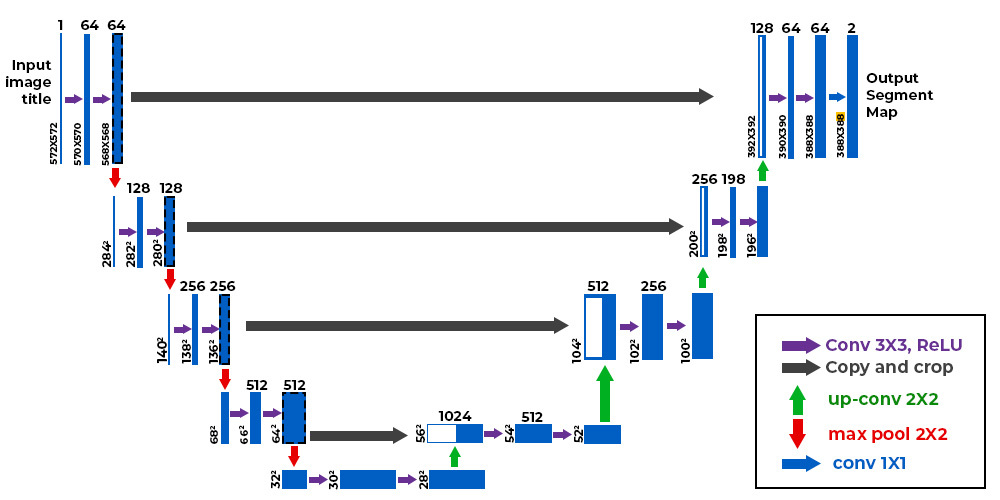
\includegraphics[width=0.7\linewidth]{Images/U-Net.jpg}
        \caption{Shema U-Net mreže~\cite{UNet}.}
        \label{fig:U-Net}
\end{figure}

Obsega skrčevalno (angl.: \textit{contracting}) pot in širitveno (angl.: \textit{expanding}) pot. Skrčevalna pot vključuje sloje kodirnika, ki identificirajo ustrezne funkcije s konvolucijskimi operacijami in postopoma abstrahirajo predstavitve vnosa. S tem zajemajo kontekstualne informacije in zmanjšujejo prostorsko ločljivost, medtem ko ekspanzivna pot vključuje sloje dekodirnika, ki dekodirajo podatke in uporabljajo informacije s krčne poti preko preskočnih (angl.: \textit{skip connections}) povezav za ustvarjanje zemljevida segmentacije. Preskočne povezave zadržijo prostorske informacije, izgubljene na poti krčenja, kar pomaga slojem dekodirnika pri natančni lokalizaciji značilnosti.


\newpage
\section{Psevdokoda algoritmov}
\label{sec:pseudocode}


\begin{figure}[ht]
    \begin{center}
    \begin{subfigure}[b]{0.9\textwidth}
    \centerline{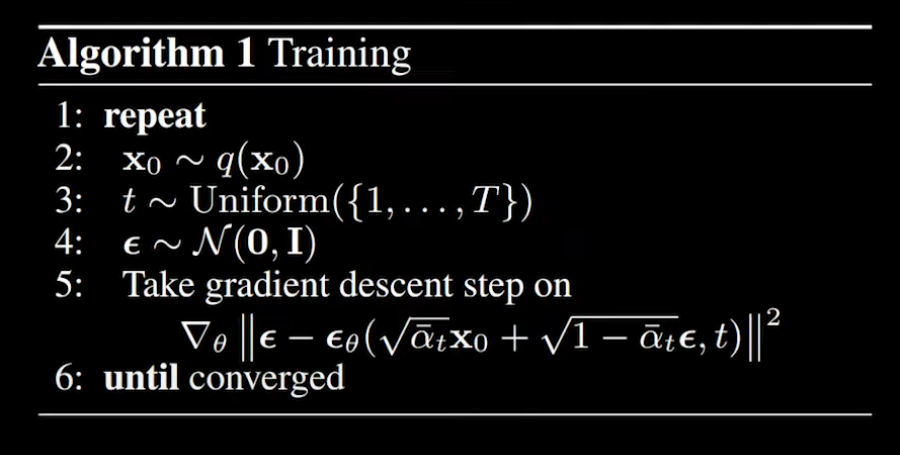
\includegraphics[width=\textwidth]{Images/ALG1.png}}
    \end{subfigure}\quad
    %\hfill
    \begin{subfigure}[b]{0.9\textwidth}
    \centerline{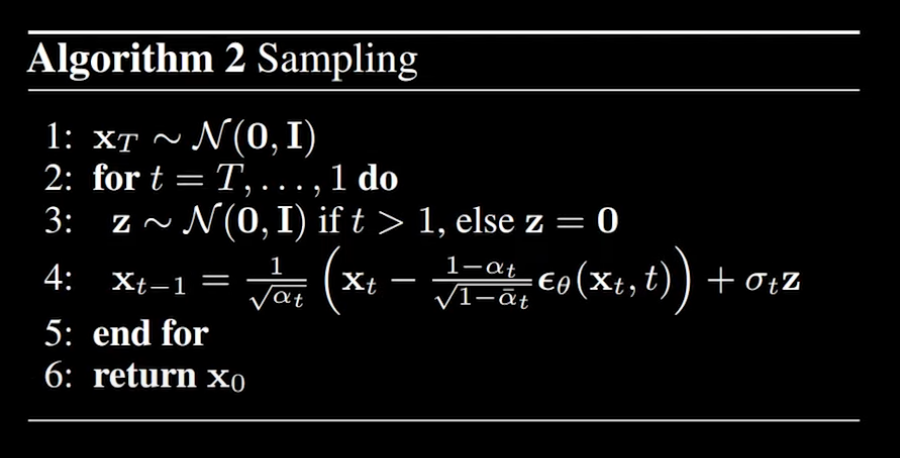
\includegraphics[width=\textwidth]{Images/ALG2.png}}
    \end{subfigure}
    
    \caption{Psevdokoda algoritma za treniranje difuzijskega modela (levo) in psevdokoda algoritma za vzorčenje z uporabo difuzijskega modela (desno). Povzeto po~\cite{DDPM}.}
    \label{fig:algorithms}
    \end{center}
    
    \vskip -0.2in
\end{figure}

\end{document}